\chapter{Reading the Paper III: The Arithmetic Information Generalizes}\label{ch:paper-arithmetic}

\begin{chapterintro}
Chapter~\ref{ch:paper-memorization} ended on a hard negative result. Fitted potentials on the Wu--Sprung background reproduce their training zeros closely, yet their predictions for zeros they were not shown are no better than the "no fluctuation" null. A skeptic could now say: perhaps nothing predicts the zeros. Perhaps zero number 401 is, for practical purposes, unpredictable from zeros $1$ to $400$, and the operators fail simply because the task is impossible.

Section~IV of the paper answers that skeptic. It has three jobs. First, it shows that the information needed to predict unseen zeros \emph{exists} and is arithmetic: a truncation of the explicit formula with zero fitted parameters predicts held-out zeros with correlation up to $+0.99$ all the way to zero $10^4$ (Table~V). Second, it separates two explanations for the operators' failure that are easy to confuse: "too few parameters" and "the wrong kind of parameters". Four controls (A, B, C1, C2 of Table~IV) settle this. Third, it checks honestly whether a fitted model with no arithmetic input that nevertheless "finds the primes" is fooling itself; this is the surrogate alignment check, which the paper labels exploratory.

This chapter teaches no new mathematics. It reads paper Sec.~IV line by line, together with the parts of Sec.~II~D, Sec.~VI and Appendix~A (steps 8, 20 and 23) that it relies on. For every claim we say what it means in plain words, which earlier chapters supply the tools, how the computation works (rerunning it at small scale with \texttt{qmnt} where feasible), and how strong it is. Where this shows up in the paper: Sec.~IV, Tables~IV and V, Eq.~(4), Fig.~1, Sec.~II~D, Sec.~VI, and Appendix~A steps 8, 20 and 23.
\end{chapterintro}

\begin{prerequisites}
\item Root finding by bracketing and Brent's method; inverting a monotone function (Chapter~\ref{ch:asymptotics}).
\item Sinusoids, phase, almost-periodic sums of incommensurate frequencies (Chapter~\ref{ch:fourier-series}).
\item Fourier resolution $\Delta\omega\approx 2\pi/T$, the periodogram, irregular sampling, phase randomization (Chapter~\ref{ch:fourier-transform}).
\item Linear least squares, the SVD, underdetermined systems, ridge regularization with filter factors $\sigma/(\sigma^2+\lambda\sigma_1^2)$ (Chapter~\ref{ch:least-squares}).
\item Primes, prime powers, the prime number theorem, the von Mangoldt function (Chapter~\ref{ch:primes}).
\item The smooth counting function $\Nsm$, smooth zeros $s_n$, mean spacing $\gap_n$, fluctuations in mean spacings (Chapter~\ref{ch:counting-zeros}).
\item The explicit formula, its truncation Eq.~(4), Landau's formula and its peaks at $\log p^m$ (Chapter~\ref{ch:explicit-formula}).
\item rms, Pearson correlation and the difference between them (Chapter~\ref{ch:probability}).
\item Training and test sets, the null model, covariate shift, inductive bias (Chapter~\ref{ch:generalization}).
\item Bootstrap intervals, surrogate data, exploratory versus confirmatory analysis (Chapter~\ref{ch:controls}).
\item Sinusoidal regression, the dense-grid and sparse-search controls, dephasing (Chapter~\ref{ch:sparse-frequency}).
\item The paper's protocol and its Sec.~III results (Chapters~\ref{ch:paper-setup} and \ref{ch:paper-memorization}).
\item First-year physics: the phase of an oscillation, and beats between two nearby frequencies.
\end{prerequisites}

%======================================================================
\section{What Section IV sets out to show}\label{sec:paper-arithmetic-aim}

Recall the situation at the end of paper Sec.~III. The fitted operators have rms errors on held-out zeros between about $0.27$ and $0.44$ mean spacings (Table~I), against a null of $0.263$ on the principal holdout, zeros 401--500 (running example RE5). Their held-out correlations with the truth hover around zero. Two very different stories could explain this:

\begin{enumerate}
\item \textbf{The "no information" story.} The fluctuations of zeros beyond 400 are not determined, in any usable way, by anything we could know. Then every model must fail, and the operators are blameless.
\item \textbf{The "wrong vocabulary" story.} The information is there, but a potential $V(x)$ expanded in a generic basis cannot express it in a form that continues past the training window.
\end{enumerate}

Section~IV is built to decide between these. Its title states the verdict: "The arithmetic information generalizes." Table~\ref{tab:paper-arithmetic-claims} lists the claims we will read, in the order of this chapter.

\begin{table}[htbp]\centering\small
\caption{The claims of paper Sec.~IV (with supporting text from Secs.~II~D and VI) read in this chapter. "Where" gives the R1 location.}\label{tab:paper-arithmetic-claims}
\begin{tabular}{p{0.6cm}p{8.2cm}p{2.6cm}}
\toprule
 & Claim (paraphrase) & Where \\
\midrule
IV.1 & The truncated explicit formula predicts unseen zeros essentially as well at $n=10^4$ as at $n=400$. & Sec.~IV, Table~V \\
IV.2 & One prime beats every fitted operator's holdout performance by a factor $\gtrsim 1.3$, with zero fitted parameters. & Sec.~IV \\
IV.3 & Twenty-five primes reach rms $0.04$--$0.07$ with correlation $+0.98$ to $+0.99$. & Sec.~IV, Table~V \\
IV.4 & The oracle is not a fair machine-learning competitor; it shows only that transferable structure exists and is arithmetic. & Secs.~II~D, IV \\
IV.5 & Control A (the oracle at a larger prime budget): going from 25 primes ($0.043$) to 300 primes, i.e.\ 900 terms, still with zero fitted parameters, the oracle improves monotonically, to $0.018$. & Sec.~IV, Table~IV \\
IV.6 & Control B: with frequencies given and amplitudes fitted, 150 coefficients give $0.028$; at 900 coefficients on 400 zeros the problem is underdetermined and the score degrades to $0.180$/$+0.78$ (root-ambiguous). & Sec.~IV, Table~IV \\
IV.7 & Control C1: a dense 900-coefficient Fourier model stays within $0.005$ of the null. & Sec.~IV, Table~IV \\
IV.8 & Control C2: a sparse search with no arithmetic input selects frequencies at $\log p^m$ and predicts at $0.034$/$+0.99$; an exploratory surrogate check supports the alignment. & Sec.~IV, App.~A step 23 \\
IV.9 & C2's skill decays with distance from the training window as its frequencies dephase. & Sec.~IV \\
IV.10 & The obstacle is the parametrization, not the parameter count. & Abstract, Secs.~IV, VI \\
\bottomrule
\end{tabular}
\end{table}

For each claim we will give (a) what it says in plain words, (b) the chapters that supply the tools, (c) the computation behind it, rerun at small scale where feasible, and (d) its strength and its limits.

\begin{pitfall}
The letters $A$ and $T$ are badly overloaded in the paper, and Sec.~IV adds to the load. In this chapter, "control A" means the oracle run with a larger prime budget. It has nothing to do with the sensitivity matrix $A_{nk}=\int|\psi_n|^2\phi_k\,\dd x$ of Sec.~II~C, nor with the non-Hermitian operator $iA$ of Sec.~II~E. Likewise $T$ here is always the length, in $t$, of the training window; it is not the second-order tensor $T^{(n)}$ of Eq.~(5), nor a Chebyshev polynomial $T_k$. When you read Sec.~IV, mentally replace "A" by "control A" and $T$ by "window length".
\end{pitfall}

\begin{keyideas}
\item Section~IV distinguishes "the information does not exist" from "the operators cannot express it".
\item It does so with one zero-parameter predictor (the oracle, Table~V) and four controls of increasing ignorance about arithmetic (A, B, C1, C2, Table~IV).
\item Every claim is measured against the same null as the operators: $0.263$ on zeros 401--500 and $0.274$ on 801--1000.
\end{keyideas}

%======================================================================
\section{The oracle and how it is scored}\label{sec:paper-arithmetic-oracle}

\subsection{The formula}

Recall from Chapter~\ref{ch:explicit-formula} that the fluctuating part of the zero-counting function is approximated by a sum over prime powers. The paper's Eq.~(4) truncates it to a prime set $P$ and to $m\le3$:
\begin{equation}
\Nfl(t) = -\frac{1}{\pi}\sum_{p\in P}\sum_{m=1}^{3}\frac{\sin(m t\log p)}{m\,p^{m/2}} .
\label{eq:paper-arithmetic-nfl}
\end{equation}
Here $t$ is height on the critical line, $p$ runs over the primes in $P$, $m$ is the power, and $\log$ is the natural logarithm. Each term is a sinusoid in $t$ with angular frequency $m\log p$ and amplitude $1/(\pi m p^{m/2})$. We will often call $w(p^m)=1/(m p^{m/2})$ the \emph{weight} of the prime power $q=p^m$; the amplitude is $w/\pi$. Recall also, from Chapter~\ref{ch:explicit-formula}, that the untruncated sum does not converge on the critical line, so Eq.~\eqref{eq:paper-arithmetic-nfl} is a heuristic approximation whose quality must be measured, not assumed. Measuring it is exactly what Table~V does.

\subsection{From formula to predicted zeros}

The smooth counting function of paper Eq.~(1) is
\begin{equation}
\Nsm(t)=\frac{t}{2\pi}\log\frac{t}{2\pi}-\frac{t}{2\pi}+\frac78 .
\label{eq:paper-arithmetic-nsm}
\end{equation}
The true counting function $N(t)$ is a staircase that jumps by $1$ at each zero. Just below $t_n$ it equals $n-1$, just above it equals $n$. The midpoint of the jump is $n-\tfrac12$. The oracle predicts the $n$-th zero as the height $t$ where the smooth-plus-fluctuating count reaches that midpoint:
\begin{equation}
\Nsm(t)+\Nfl(t) = n-\tfrac12 .
\label{eq:paper-arithmetic-level}
\end{equation}
We call Eq.~\eqref{eq:paper-arithmetic-level} the \emph{level equation}. Appendix~A step 8 records how it is solved: Brent's method (Chapter~\ref{ch:asymptotics}) on a bracket of $\pm3$ mean spacings around the smooth zero $s_n$, with the bracket expanded if the function has the same sign at both ends. Recall that $s_n$ solves $\Nsm(s_n)=n-\tfrac12$ and that the local mean spacing is
\begin{equation}
\gap_n = \frac{\dd s_n}{\dd n} = \frac{2\pi}{\log(s_n/2\pi)} .
\label{eq:paper-arithmetic-gap}
\end{equation}

\begin{checkpoint}
The oracle's prediction of zero $n$ uses the index $n$, the smooth zero $s_n$ (to place the bracket) and the prime set $P$. Does it use any computed zeta zero at all?
\end{checkpoint}
\checkanswer{No. $s_n$ comes from Eq.~\eqref{eq:paper-arithmetic-nsm} alone, and $\Nfl$ from the primes alone. No zero, in-sample or held-out, enters the prediction. That is why the paper can say the oracle has "zero fitted parameters" and why it needs no training window.}

\subsection{How predictions are scored}

The score is the one used everywhere in the paper (Chapter~\ref{ch:paper-setup}). For each held-out index $n$, convert a zero $t$ into a fluctuation in mean spacings,
\begin{equation}
f_n(t) = \frac{t-s_n}{\gap_n} .
\label{eq:paper-arithmetic-fluct}
\end{equation}
The true fluctuation is $f_n(t_n)$ and the predicted one is $f_n(t_n^{\rm pred})$. The rms of their difference over the holdout is the "rms"; the Pearson correlation between the two sequences is the "corr". The null predicts $t_n=s_n$, so its fluctuation is $0$ and its rms is the rms of the true fluctuations themselves: $0.263$ on zeros 401--500.

\subsection{What the oracle's prediction is, in mean spacings}

It helps to see what Eq.~\eqref{eq:paper-arithmetic-level} does to the fluctuation. Write the predicted zero as $t=s_n+\delta$. Taylor's theorem with remainder (Chapter~\ref{ch:asymptotics}) applied to $\Nsm$ gives
\begin{align}
\Nsm(s_n+\delta) &= \Nsm(s_n) + \delta\,\Nsm'(s_n) + \tfrac12\delta^2\,\Nsm''(\xi)
\quad\text{(some $\xi$ between $s_n$ and $s_n+\delta$)}\nonumber\\
&= n-\tfrac12 + \frac{\delta}{\gap_n} + \tfrac12\delta^2\,\Nsm''(\xi).
\label{eq:paper-arithmetic-taylor}
\end{align}
The second line used two facts. First, $\Nsm(s_n)=n-\tfrac12$ by definition of $s_n$. Second, differentiating Eq.~\eqref{eq:paper-arithmetic-nsm},
\begin{align}
\Nsm'(t) &= \frac{1}{2\pi}\log\frac{t}{2\pi} + \frac{t}{2\pi}\cdot\frac{1}{t} - \frac{1}{2\pi}
\quad\text{(product rule on the first term)}\nonumber\\
&= \frac{1}{2\pi}\log\frac{t}{2\pi},
\label{eq:paper-arithmetic-nsmprime}
\end{align}
which is exactly $1/\gap_n$ at $t=s_n$ by Eq.~\eqref{eq:paper-arithmetic-gap}. Differentiating once more gives $\Nsm''(t)=1/(2\pi t)$.

Now substitute Eq.~\eqref{eq:paper-arithmetic-taylor} into the level equation \eqref{eq:paper-arithmetic-level}:
\begin{align}
n-\tfrac12 + \frac{\delta}{\gap_n} + \tfrac12\delta^2\Nsm''(\xi) + \Nfl(s_n+\delta) &= n-\tfrac12\nonumber\\
\frac{\delta}{\gap_n} &= -\Nfl(s_n+\delta) - \tfrac12\delta^2\Nsm''(\xi).
\label{eq:paper-arithmetic-exactfluct}
\end{align}
The left side is the predicted fluctuation $f_n$ of Eq.~\eqref{eq:paper-arithmetic-fluct}. The curvature term is tiny: with $\delta\approx\gap_n\approx1.34$ and $t\approx680$ (the top of the training window), it is $\tfrac12(1.3414)^2/(2\pi\cdot680)\approx 2\times10^{-4}$ mean spacings. So, to that accuracy,
\begin{equation}
f_n^{\rm pred} \approx -\Nfl\bigl(t_n^{\rm pred}\bigr).
\label{eq:paper-arithmetic-predfluct}
\end{equation}
\textbf{In mean spacings, the oracle's predicted fluctuation is minus the prime sum evaluated at the predicted zero.} The same argument applied to a true zero shows that the true fluctuation $f_n(t_n)$ is, to the same accuracy, $-y_n$ with
\begin{equation}
y_n = n-\tfrac12-\Nsm(t_n),
\label{eq:paper-arithmetic-yn}
\end{equation}
the amount by which the smooth count misses the midpoint at the true zero. This $y_n$ will reappear as the training target of every fitted control.

\begin{sample}{One oracle step by hand}
Use only the prime $2$ (the running example RE2, $m=1,2,3$). Pretend that $s=680$ is a smooth zero, so that the target count is $\Nsm(680)$. (The index would not be an integer; the algebra does not care.) Find the oracle's predicted shift $\delta$ (a) by neglecting the variation of $\Nfl$ over the shift, (b) by one Newton step on the full level equation, and (c) exactly.

\textbf{Step 1: evaluate $\Nfl$ at $s$.} The phases are $m\cdot680\log2$ reduced modulo $2\pi$. With $\log2=0.693147$, $680\log 2 = 471.34008$, and $75\cdot2\pi=471.23890$, so the $m=1$ phase is $0.10118$. Doubling and tripling (and removing $150\cdot2\pi$ and $225\cdot2\pi$) give $0.20237$ and $0.30355$. Then
\[
\Nfl(680) = -\frac1\pi\Bigl[\frac{\sin 0.10118}{\sqrt2}+\frac{\sin0.20237}{2\cdot2}+\frac{\sin0.30355}{3\cdot2^{3/2}}\Bigr]
= -\frac{0.15690}{\pi} = -0.0499 .
\]

\textbf{Step 2: the mean spacing and slope of $\Nsm$.} By Eq.~\eqref{eq:paper-arithmetic-nsmprime}, $\Nsm'(680)=\log(108.225)/2\pi = 0.7455$, so $\gap = 1/0.7455 = 1.3414$.

\textbf{Step 3: approximation (a).} Neglect the change of $\Nfl$ and the curvature in Eq.~\eqref{eq:paper-arithmetic-exactfluct}: $\delta_a = -\gap\cdot\Nfl(680) = 1.3414\times0.0499 = 0.0670$.

\textbf{Step 4: approximation (b).} The full level function is $G(t)=\Nsm(t)-\Nsm(680)+\Nfl(t)$ with $G(680)=-0.0499$. Its slope is $G'(680)=\Nsm'(680)+\Nfl'(680)$, where
\[
\Nfl'(t) = -\frac{1}{\pi}\sum_{m=1}^3 \frac{\log 2\,\cos(m t\log2)}{2^{m/2}} ,
\qquad \Nfl'(680) = -0.3377 .
\]
One Newton step gives $\delta_b = -G(680)/G'(680) = 0.0499/(0.7455-0.3377) = 0.122$.

\textbf{Step 5: exact root.} Brent's method on $[680-3\gap,\,680+3\gap]$ (see CHECKS) gives the root at $\delta_c = 0.120$, that is, a predicted fluctuation of $0.120/1.3414 = 0.090$ mean spacings. As Eq.~\eqref{eq:paper-arithmetic-predfluct} promises, this is $-\Nfl$ at the root, not at $s$.

\[
\boxed{\delta_a = 0.0670,\quad \delta_b = 0.122,\quad \delta_c = 0.120\ \ (0.090\ \text{mean spacings})}
\]
The lesson: the slope of the prime sum, $-0.34$, is not small next to the slope of the smooth count, $0.75$. Neglecting it nearly halves the shift. That is why the paper solves the level equation by root finding instead of stepping once from $s_n$.
\end{sample}

\subsection{Is the root unique?}

Brent's method returns one root of the level equation in its bracket. If $G(t)=\Nsm(t)+\Nfl(t)-(n-\tfrac12)$ is strictly increasing, there is exactly one. A sufficient condition is that $|\Nfl'(t)|<\Nsm'(t)$ everywhere near the bracket. Differentiating Eq.~\eqref{eq:paper-arithmetic-nfl} term by term,
\begin{equation}
\Nfl'(t) = -\frac{1}{\pi}\sum_{p\in P}\sum_{m=1}^3 \frac{m\log p\,\cos(m t\log p)}{m p^{m/2}}
= -\frac{1}{\pi}\sum_{p\in P}\sum_{m=1}^3 \frac{\log p\,\cos(m t\log p)}{p^{m/2}} ,
\label{eq:paper-arithmetic-dnfl}
\end{equation}
and since $|\cos|\le1$,
\begin{equation}
|\Nfl'(t)| \le B_P \equiv \frac{1}{\pi}\sum_{p\in P}\log p\,\bigl(p^{-1/2}+p^{-1}+p^{-3/2}\bigr).
\label{eq:paper-arithmetic-bound}
\end{equation}
This bound is the worst case, reached only if all cosines equal $1$ at once. It is useful because it is simple.

\begin{sample}{When is the oracle's root guaranteed unique?}
Compute $B_P$ for $P=\{2\}$ and for the six primes $P=\{2,3,5,7,11,13\}$, and find the heights above which $B_P<\Nsm'(t)$.

\textbf{Step 1: $P=\{2\}$.} $\log2\,(0.70711+0.5+0.35355)=0.69315\times1.56066=1.08178$, so $B_{\{2\}}=1.08178/\pi=0.3443$.

\textbf{Step 2: threshold for $\{2\}$.} By Eq.~\eqref{eq:paper-arithmetic-nsmprime} we need $\log(t/2\pi)/2\pi>0.3443$, that is $\log(t/2\pi)>2.1636$, so $t/2\pi>e^{2.1636}=8.702$ and $t>54.7$.

\textbf{Step 3: six primes.} The six contributions $\log p\,(p^{-1/2}+p^{-1}+p^{-3/2})$ are $1.0818,\ 1.2119,\ 1.1856,\ 1.1185,\ 1.0067,\ 0.9634$; their sum is $6.568$, so $B_6 = 6.568/\pi = 2.09$.

\textbf{Step 4: threshold for six primes.} We need $\log(t/2\pi)>2\pi\times2.09=13.14$, that is $t>2\pi e^{13.14}\approx3.2\times10^6$.

\[
\boxed{B_{\{2\}}=0.344\ \Rightarrow\ \text{unique root for } t>54.7;\qquad B_6=2.09\ \Rightarrow\ \text{guaranteed only for } t\gtrsim3.2\times10^6}
\]
The worst-case bound is far from typical. Because the frequencies are incommensurate, the cosines in Eq.~\eqref{eq:paper-arithmetic-dnfl} do not line up, and the rms of $\Nfl'$ over $t$ is $\frac1\pi\bigl[\sum_p(\log p)^2\sum_m \frac{1}{2p^m}\bigr]^{1/2}=0.415$ for six primes (Problem~\ref{prob:paper-arithmetic-rmsslope} asks you to derive this formula). That is well below $\Nsm'\approx0.75$ at the heights of the paper. So failure of monotonicity is possible but rare for the oracle; the paper reports root ambiguity only for one fitted row of Table~IV, which we meet in \cref{sec:paper-arithmetic-B}.
\end{sample}

\subsection{Rerunning Table V at small scale}

The listing below recomputes the first row of paper Table~V. It uses \texttt{qmnt.first\_primes(k)} for the first $k$ primes, \texttt{qmnt.oracle\_zeros} for the bracketed Brent solution of Eq.~\eqref{eq:paper-arithmetic-level}, and \texttt{qmnt.score} for the paper's scoring.

\begin{pycode}
import numpy as np, qmnt
n = np.arange(401, 501)                 # held-out indices (RE5)
t_true = qmnt.zeros(500)[400:500]       # t_401 ... t_500
null = qmnt.rms(qmnt.fluct(t_true, n))  # the "no fluctuation" prediction
print("null", round(null, 3))
for k in (1, 3, 6, 25):                 # prime budgets of Table V
    P = qmnt.first_primes(k)
    t_pred = qmnt.oracle_zeros(n, P, mmax=3)
    r, c = qmnt.score(t_pred, n)        # rms (mean spacings), Pearson corr
    print(k, "primes:", round(r, 3), round(c, 2))
\end{pycode}

Running it reproduces the paper's row to the printed precision: null $0.263$; one prime $0.198/+0.66$; three primes $0.116/+0.90$; six primes $0.074/+0.96$; twenty-five primes $0.043/+0.99$ (all verified in CHECKS). Setting \texttt{n = np.arange(1001, 2001)} and \texttt{t\_true = qmnt.zeros(2000)[1000:2000]} reproduces the third row, for instance $0.091/+0.95$ for six primes. \cref{fig:paper-arithmetic-oraclefit} shows the six-prime prediction against the truth around the train/test boundary used in paper Fig.~1.

\begin{figure}[htbp]\centering
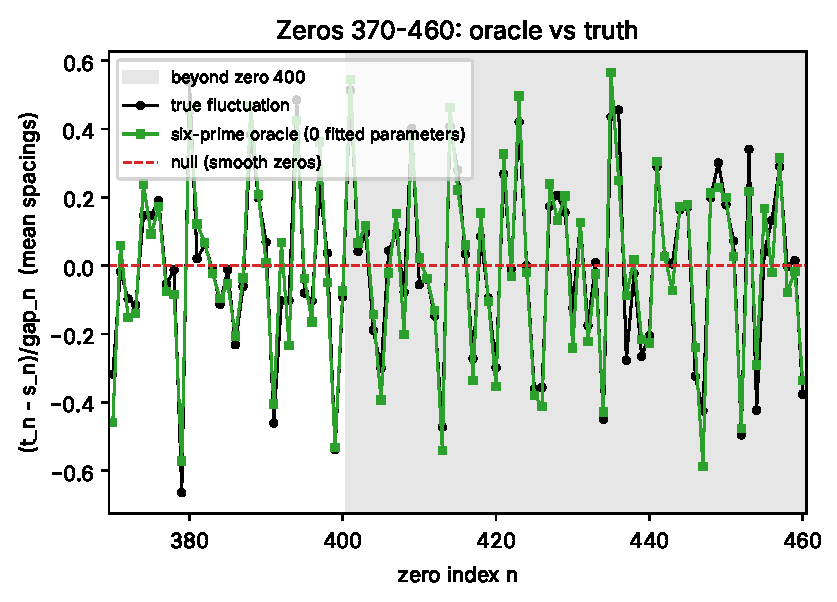
\includegraphics[width=0.85\linewidth]{figs/paper-arithmetic_oraclefit.pdf}
\caption{A small-scale rerun of the oracle half of paper Fig.~1. Black circles: true fluctuations $(t_n-s_n)/\gap_n$ of zeros 370--460, in mean spacings. Green squares: the six-prime oracle of Eq.~\eqref{eq:paper-arithmetic-nfl} ($p\le13$, $m\le3$), obtained by solving the level equation \eqref{eq:paper-arithmetic-level} with zero fitted parameters. Dashed red: the null (no fluctuation). The shaded region, beyond zero 400, is where the paper's fitted operator is held out; the oracle has no training window, so nothing changes at the boundary. The paper reports held-out correlations $+0.96$ (oracle) and $-0.07$ (operator) for this figure.}
\label{fig:paper-arithmetic-oraclefit}
\end{figure}

\begin{keyideas}
\item The oracle solves $\Nsm(t)+\Nfl(t)=n-\tfrac12$ with no fitted parameters and no zero data, Eq.~\eqref{eq:paper-arithmetic-level}.
\item In mean spacings its predicted fluctuation is $-\Nfl$ at the predicted zero, Eq.~\eqref{eq:paper-arithmetic-predfluct}; the true fluctuation is $-y_n$, Eq.~\eqref{eq:paper-arithmetic-yn}.
\item The slope of $\Nfl$ is comparable with that of $\Nsm$, so the level equation must be solved, not linearized; uniqueness of the root is guaranteed by the simple bound \eqref{eq:paper-arithmetic-bound} for one prime but not for six.
\item Table~V's oracle rows are reproducible in a few seconds with \texttt{qmnt}.
\end{keyideas}

%======================================================================
\section{Table V: prediction through zero ten thousand}\label{sec:paper-arithmetic-tablev}

\subsection{What the table says}

Table~\ref{tab:paper-arithmetic-tablev} copies paper Table~V. Every entry has zero fitted parameters. Each cell is "rms / corr" on the stated holdout.

\begin{table}[htbp]\centering\small
\caption{Paper Table~V, quoted exactly: the oracle of Eq.~\eqref{eq:paper-arithmetic-nfl}, rms / correlation on held-out zeros, for prime budgets $\{2\}$, the first 3, 6 and 25 primes.}\label{tab:paper-arithmetic-tablev}
\begin{tabular}{lccccc}
\toprule
holdout & null & $\{2\}$ & 3 primes & 6 primes & 25 primes \\
\midrule
401--500 & 0.263 & 0.198 / $+0.66$ & 0.116 / $+0.90$ & 0.074 / $+0.96$ & 0.043 / $+0.99$ \\
501--1000 & 0.270 & 0.208 / $+0.64$ & 0.127 / $+0.88$ & 0.083 / $+0.95$ & 0.050 / $+0.99$ \\
1001--2000 & 0.279 & 0.219 / $+0.62$ & 0.139 / $+0.87$ & 0.091 / $+0.95$ & 0.054 / $+0.98$ \\
2001--5000 & 0.288 & 0.232 / $+0.59$ & 0.156 / $+0.84$ & 0.107 / $+0.93$ & 0.060 / $+0.98$ \\
5001--10000 & 0.296 & 0.242 / $+0.58$ & 0.169 / $+0.82$ & 0.119 / $+0.92$ & 0.067 / $+0.98$ \\
\bottomrule
\end{tabular}
\end{table}

Read across a row: more primes, better prediction, with no exception. Read down a column: the rms grows slowly with height. Claim IV.3 is the last column: rms $0.043$ to $0.067$, which the paper rounds to "$0.04$--$0.07$", with correlation $+0.98$ to $+0.99$.

Claim IV.1 says the formula predicts "essentially as well at $n=10^4$ as at $n=400$". To weigh the word "essentially", divide each rms by the null of its row. The result is Table~\ref{tab:paper-arithmetic-ratio}: the fraction of the null error that remains.

\begin{table}[htbp]\centering\small
\caption{Ratio rms/null computed from Table~\ref{tab:paper-arithmetic-tablev} (our arithmetic, checked in CHECKS). Smaller is better; 1 would mean no skill.}\label{tab:paper-arithmetic-ratio}
\begin{tabular}{lcccc}
\toprule
holdout & $\{2\}$ & 3 primes & 6 primes & 25 primes \\
\midrule
401--500 & 0.75 & 0.44 & 0.28 & 0.16 \\
501--1000 & 0.77 & 0.47 & 0.31 & 0.19 \\
1001--2000 & 0.78 & 0.50 & 0.33 & 0.19 \\
2001--5000 & 0.81 & 0.54 & 0.37 & 0.21 \\
5001--10000 & 0.82 & 0.57 & 0.40 & 0.23 \\
\bottomrule
\end{tabular}
\end{table}

Two honest readings are possible. By correlation, skill is nearly constant: $+0.99$ to $+0.98$ at 25 primes. By the rms ratio, it drifts upward, from $0.16$ to $0.23$ at 25 primes. The paper's caption to Table~V gives the reason for the drift: "The mild growth at fixed prime budget mirrors the growth of the null and the increasing number of arithmetically relevant primes at height; relative skill is nearly constant." Dividing by the null removes the first effect. What remains in Table~\ref{tab:paper-arithmetic-ratio} is the second: at greater heights, a fixed set of primes captures a smaller share of the fluctuation because more primes contribute appreciably. "Nearly constant" is the paper's wording, and it is a fair summary of a ratio that changes by about a factor $1.4$ over a factor $25$ in height. \cref{fig:paper-arithmetic-tablev} shows both views.

\begin{figure}[htbp]\centering
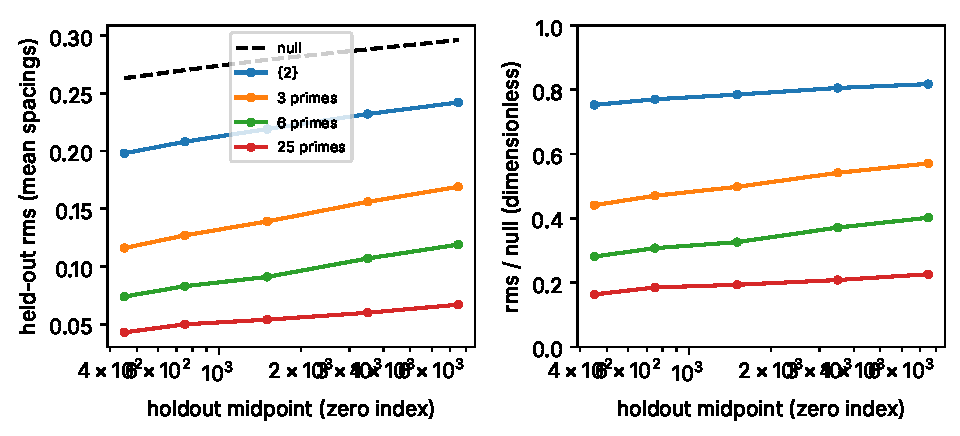
\includegraphics[width=0.95\linewidth]{figs/paper-arithmetic_tablev.pdf}
\caption{Paper Table~V plotted against the midpoint of each holdout (log scale). Left: rms in mean spacings for each prime budget, with the null (dashed). Right: rms divided by the null, Table~\ref{tab:paper-arithmetic-ratio}. Every curve stays far below the null through zero $10^4$; the slow upward drift at fixed budget reflects the growing number of relevant primes at height.}
\label{fig:paper-arithmetic-tablev}
\end{figure}

\begin{beyond}
\textbf{Why the null grows, and why more primes matter higher up.} A theorem of Selberg (his central limit theorem for $S(t)$; see the discussion in \cite{titchmarsh}) states that, as $t\to\infty$, $S(t)$ divided by $\sqrt{\tfrac{1}{2\pi^2}\log\log t}$ becomes distributed like a standard Gaussian. We take this on trust; its proof is beyond this book. A note on units: $S(t)$ is measured in counts, while the paper's fluctuations are measured in mean spacings. To leading order these are the same: by Eqs.~\eqref{eq:paper-arithmetic-predfluct} and \eqref{eq:paper-arithmetic-yn}, a count offset $y_n$ at a zero corresponds to a height offset of about $y_n\gap_n$, which is $y_n$ mean spacings, because the local density of zeros is $1/\gap_n$. So the variance of $S$ applies directly to the fluctuations in mean spacings, up to the small curvature and slope corrections neglected in those equations. Heuristically, the variance $\tfrac{1}{2\pi^2}\log\log t$ matches the variance $\sum_{p\le x}\tfrac{1}{2\pi^2 p}\approx\tfrac{1}{2\pi^2}\log\log x$ of the $m=1$ prime terms (each sinusoid of amplitude $1/(\pi\sqrt p)$ has mean square $1/(2\pi^2p)$), with an effective prime cutoff $x$ that grows with $t$. This is a heuristic, not a derivation, but it explains both trends in Table~V: the null grows very slowly, like $\sqrt{\log\log t}$, and a fixed prime budget covers a shrinking part of the variance. Problem~\ref{prob:paper-arithmetic-selberg} compares the predicted growth with the table.
\end{beyond}

\subsection{"One prime beats every fitted operator"}

Claim IV.2 is a comparison between Table~V and Table~I.

\begin{sample}{The factor 1.3}
The fitted operators' OOS rms values in paper Table~I are $0.317,\ 0.320,\ 0.273,\ 0.274,\ 0.369,\ 0.271,\ 0.265,\ 0.313,\ 0.439,\ 0.370,\ 0.279,\ 0.302$. The one-prime oracle scores $0.198$ on zeros 401--500 and $0.208$ on 501--1000 (Table~V). Check the paper's "factor $\gtrsim1.3$".

\textbf{Step 1: the best operator.} The smallest value in the list is $0.265$ (scale 1, fit 1--400, $M=400$, ridge $\mu=0.3$). Its holdout is 401--500.

\textbf{Step 2: compare on the same holdout.} $0.265/0.198 = 1.34$.

\textbf{Step 3: the best scale-2 operator.} The smallest scale-2 value is $0.279$ (holdout 801--1000). The closest Table~V row is 501--1000, where one prime gives $0.208$; $0.279/0.208=1.34$.

\[
\boxed{\text{smallest ratio}\approx1.34\ \ (\gtrsim1.3)}
\]
Two caveats keep this honest. The scale-2 comparison uses neighboring rather than identical holdouts, so it is approximate. And the operators' holdouts for fits on zeros 1--300, 1--350 and 1--450 differ from 401--500; but each of those operators scores $\ge0.273$, and every Table~V entry for one prime is $\le0.242$, so the comparison holds whichever row you use.
\end{sample}

\subsection{rms and correlation tell different stories}

Throughout Table~IV you will want to read rms and correlation together. Chapter~\ref{ch:probability} showed that they measure different things. Here is the quantitative link we will use repeatedly.

Let $Y_n$ be the true fluctuations on a holdout and $P_n$ the predicted ones, with standard deviations $\sigma_Y,\sigma_P$ and correlation $\rho$. The mean squared error is
\begin{align}
\overline{(P-Y)^2} &= \mathrm{var}(P-Y) + \bigl(\overline{P-Y}\bigr)^2
\quad\text{(variance plus squared mean)}\nonumber\\
&\ge \mathrm{var}(P-Y)
= \sigma_P^2+\sigma_Y^2-2\rho\,\sigma_P\sigma_Y .
\label{eq:paper-arithmetic-mse}
\end{align}
For $\rho>0$, the right side is a quadratic in $\sigma_P$ with minimum at $\sigma_P=\rho\sigma_Y$ (set its derivative $2\sigma_P-2\rho\sigma_Y$ to zero). Substituting,
\begin{equation}
\overline{(P-Y)^2}\ \ge\ \rho^2\sigma_Y^2+\sigma_Y^2-2\rho^2\sigma_Y^2 = \sigma_Y^2(1-\rho^2),
\qquad\text{so}\qquad
\mathrm{rms} \ge \sigma_Y\sqrt{1-\rho^2}.
\label{eq:paper-arithmetic-rmsbound}
\end{equation}
The null's rms is $\sqrt{\overline{Y^2}}$, which equals $\sigma_Y$ when the true fluctuations average to zero. They nearly do, so we use the null as an approximation to $\sigma_Y$. (What is neglected: the squared mean of $Y$ over the holdout, which is small compared with $\sigma_Y^2$.)

\begin{sample}{Reading a correlation off an rms, and vice versa}
(a) Control C1 has correlation $+0.28$ on zeros 401--500 (Table~IV). What is the best rms any prediction with that correlation could have? (b) Control B with 25 primes has rms $0.028$ on the same holdout. What correlation does that imply?

\textbf{Step 1: (a).} With $\sigma_Y\approx0.263$ and $\rho=0.28$, Eq.~\eqref{eq:paper-arithmetic-rmsbound} gives $0.263\sqrt{1-0.0784}=0.263\times0.960=0.252$.

\textbf{Step 2: compare.} C1 scores $0.258$, close to this best case. C1's predictions are shrunk to small amplitude, near the optimal $\sigma_P=\rho\sigma_Y$, so its rms is near the null even though its correlation is not zero.

\textbf{Step 3: (b).} Invert Eq.~\eqref{eq:paper-arithmetic-rmsbound}: $\rho\ge\sqrt{1-(\mathrm{rms}/\sigma_Y)^2}=\sqrt{1-(0.028/0.263)^2}=\sqrt{1-0.0113}=0.994$.

\[
\boxed{\text{(a) best rms}\approx0.252;\qquad\text{(b) } \rho\gtrsim0.994}
\]
Part (b) explains why Table~IV prints "$+0.99$" next to $0.028$ and "$+1.00$" next to $0.018$: at such small errors the correlation is forced toward 1, and two-decimal rounding cannot show the difference.
\end{sample}

\begin{checkpoint}
A model has held-out correlation $+0.28$ and rms almost equal to the null. Is it useless?
\end{checkpoint}
\checkanswer{Not entirely. A correlation of $+0.28$ means its predictions point weakly in the right direction; Eq.~\eqref{eq:paper-arithmetic-rmsbound} shows that even the best scaling of such a prediction leaves an rms of about $0.96$ times the null. So it carries a small amount of information but removes almost none of the error. This is the situation of control C1.}

\begin{keyideas}
\item Table~V: more primes always help, and skill persists through zero $10^4$; correlation is nearly constant, the rms ratio drifts mildly upward (Table~\ref{tab:paper-arithmetic-ratio}).
\item One prime beats the best fitted operator by a factor of about $1.34$ (Claim IV.2).
\item rms $\ge\sigma_Y\sqrt{1-\rho^2}$, Eq.~\eqref{eq:paper-arithmetic-rmsbound}: a weak correlation cannot produce a small rms, and a small rms forces a correlation near 1.
\end{keyideas}

%======================================================================
\section{Three levels of supplied information}\label{sec:paper-arithmetic-levels}

\subsection{Why the oracle alone is not enough}

The paper is explicit that the oracle "is not a fair ML competitor (it encodes the known functional form); its role is informational" (Sec.~II~D), and again in Sec.~IV: "it is given the functional form, so this comparison shows only that transferable structure exists and is arithmetic." The operators were given a background potential and a basis; the oracle was given the answer's shape. A critic could therefore say: of course a model told the answer's form wins. Claim IV.4 concedes this and the controls are designed to answer the critic.

The paper organizes all models "by the information supplied, at three levels":
\begin{enumerate}
\item[(i)] the arithmetic frequencies $m\log p$ supplied (the oracle, control A, and control B with fitted amplitudes);
\item[(ii)] no arithmetic frequencies, but sparsity in $t$-frequency supplied (C2);
\item[(iii)] a generic basis with no such prior (the dense Fourier model C1, and the fitted potentials).
\end{enumerate}
\cref{fig:paper-arithmetic-ladder} summarizes where each model lands.

\begin{figure}[htbp]\centering
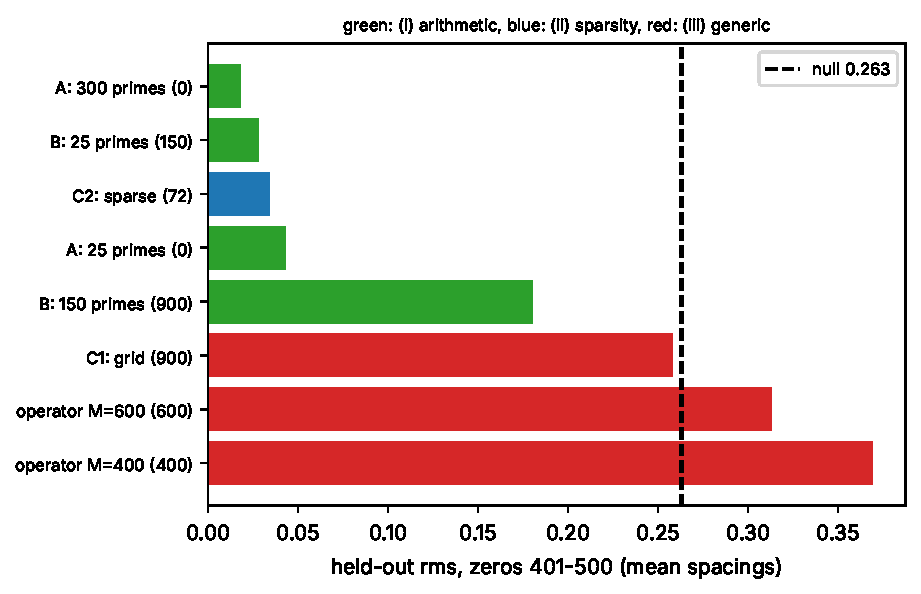
\includegraphics[width=0.85\linewidth]{figs/paper-arithmetic_ladder.pdf}
\caption{The three levels of supplied information of paper Sec.~IV, with held-out rms on zeros 401--500 from paper Table~IV (null $0.263$). Level (i) is given the arithmetic frequencies; level (ii) is told only that the fluctuation is a sum of few sinusoids; level (iii) gets a generic basis. Skill tracks the prior, not the number of fitted parameters.}
\label{fig:paper-arithmetic-ladder}
\end{figure}

\subsection{The common shape of the fitted controls}

All three fitted controls (B, C1, C2) are described in Sec.~II~D ("Fitted sinusoidal controls") as having the shape
\begin{equation}
\Nsm(t)+F(t)=n-\tfrac12,\qquad F(t)=\sum_j\bigl[a_j\sin(\omega_j t)+b_j\cos(\omega_j t)\bigr],
\label{eq:paper-arithmetic-F}
\end{equation}
"trained by least squares on $y_n=n-\tfrac12-\Nsm(t_n)$ at the training zeros only, and scored exactly as the oracle." Line by line:

\begin{itemize}
\item \emph{Shape.} Eq.~\eqref{eq:paper-arithmetic-F} is the level equation \eqref{eq:paper-arithmetic-level} with $\Nfl$ replaced by a general sum of sinusoids $F$. The oracle is the special case $\omega_j=m\log p$, $a_j=-1/(\pi m p^{m/2})$, $b_j=0$.
\item \emph{Target.} By Eq.~\eqref{eq:paper-arithmetic-yn}, $y_n$ is what $F(t_n)$ would have to be for the level equation to hold exactly at the true zero $t_n$. Fitting $F(t_n)\approx y_n$ at training zeros is the natural regression.
\item \emph{Linear in the amplitudes.} Once the frequencies $\omega_j$ are fixed, $F(t_n)$ is a linear combination of the known numbers $\sin(\omega_jt_n)$ and $\cos(\omega_jt_n)$. Stack them into a design matrix $X$ with rows indexed by training zeros and columns by $(j,\sin)$ and $(j,\cos)$. The fit is then the linear least-squares problem $X\theta\approx y$ of Chapter~\ref{ch:least-squares}, with $\theta=(a_1,\dots,b_1,\dots)$.
\item \emph{Ridge.} Appendix~A step 20 gives the ridge filter $\Sigma/(\Sigma^2+\lambda\Sigma_1^2)$: if $X=U\Sigma V^\top$ is the SVD with largest singular value $\sigma_1$, the solution is $\theta=V\,\mathrm{diag}\bigl(\sigma_i/(\sigma_i^2+\lambda\sigma_1^2)\bigr)U^\top y$. The grid of strengths is "$\lambda=10^{-8},\dots,10^{3}$ in half decades": exponents $-8,-7.5,\dots,3$, which is $23$ values.
\item \emph{Selection.} "Ridge strength and $K$ are chosen by a forward split inside the training window (first 75\% fit, last 25\% validate), after which the model is refitted on the whole training window; held-out zeros are not used before scoring." For 400 training zeros: fit 1--300, validate 301--400, pick the best $\lambda$ (and, for C2, $K$), then refit on 1--400. The forward split imitates, inside the training window, the forward extrapolation that the real test will demand (Chapter~\ref{ch:generalization}).
\item \emph{Leakage test.} Appendix~A step 20 adds: "Overwriting held-out data with noise before fitting leaves all fitted coefficients bit-identical." This is a direct, mechanical proof that no held-out zero influences any fitted number.
\end{itemize}

\begin{sample}{Counting parameters and equations}
For each model of Table~IV, count fitted real parameters and compare with the number of training zeros.

\textbf{Step 1: control A.} Three powers $m$ for each of 300 primes give $900$ terms, all with fixed amplitudes: $0$ fitted. The 300th prime is $1987$, so the highest frequency is $3\log1987=22.78$.

\textbf{Step 2: control B, 25 primes.} The 25th prime is $97$. There are $25\times3=75$ frequencies, each with a sine and a cosine amplitude: $150$ parameters, against $400$ training zeros (or $800$).

\textbf{Step 3: control B, 150 primes.} The 150th prime is $863$: $150\times3\times2=900$ parameters against $400$ zeros. The system $X\theta=y$ has more unknowns than equations, so (Chapter~\ref{ch:least-squares}) its exact solutions form a family of dimension at least $900-400=500$. With $800$ zeros it is still underdetermined, by at least $100$.

\textbf{Step 4: C1.} $450$ frequencies, two amplitudes each: $900$, underdetermined in the same way.

\textbf{Step 5: C2.} $K$ frequencies, each with a frequency, a sine and a cosine amplitude: $3K$. With $K=24$, $72$; with $K=43$, $129$. These are the "72, 129" of Table~IV.

\[
\boxed{A:0;\quad B_{25}:150;\quad B_{150}:900;\quad C1:900;\quad C2:72\ \text{or}\ 129}
\]
\end{sample}

\begin{keyideas}
\item The fitted controls replace $\Nfl$ by a sum of sinusoids $F$ fitted to $y_n=n-\tfrac12-\Nsm(t_n)$, Eq.~\eqref{eq:paper-arithmetic-F}.
\item With frequencies fixed, the fit is linear least squares with ridge; strength (and $K$) are chosen by a 75/25 forward split inside the training window.
\item The controls span parameter counts from 0 to 900 and priors from "exact arithmetic" to "generic". That design lets the paper vary count and prior separately.
\end{keyideas}

%======================================================================
\section{Control A: the oracle with a bigger budget}\label{sec:paper-arithmetic-A}

\textbf{(a) Plain words.} Table~V stops at 25 primes. Control A asks what happens at the same \emph{nominal} budget as the largest operator fit, 900 terms, with still nothing fitted. Answer (Sec.~IV): "the oracle improves monotonically, to $0.018$ on zeros 401--500." Table~IV adds $0.020/+1.00$ on 801--1000 and the bootstrap interval $[0.015, 0.020]$ on 401--500.

\textbf{(b) Tools.} The explicit formula and its truncation (Chapter~\ref{ch:explicit-formula}); bootstrap intervals (Chapter~\ref{ch:controls}).

\textbf{(c) Computation.} The same loop as in \cref{sec:paper-arithmetic-oracle} with \texttt{qmnt.first\_primes(300)}. The cost is 900 sines per evaluation of $\Nfl$, still trivial.

\textbf{(d) Strength and limits.} Control A addresses one specific objection: that the operators lose only because they have fewer "terms". At these heights the oracle with 900 terms is better than with 75 terms (25 primes), so a large term count is not, in itself, harmful when the terms have the right form. Notice too that A involves no fitting, so it cannot overfit in the statistical sense: no parameter is tuned to the training zeros. That does not make more terms automatically better. On the critical line the full series does not converge (Chapter~\ref{ch:explicit-formula}), so whether adding terms helps is an empirical question, answered affirmatively at these heights by Tables~IV and V; it is not a theorem. The word "monotonically" refers to intermediate budgets that the paper does not tabulate; we take it as reported.

\begin{pitfall}
Do not read control A's $0.018$ as "900 parameters generalize". Control A has 900 \emph{terms} and $0$ fitted parameters. The informative comparison for parameter count is between the fitted models (B, C1, C2, and the operators).
\end{pitfall}

%======================================================================
\section{Control B: arithmetic frequencies, fitted amplitudes}\label{sec:paper-arithmetic-B}

\subsection{The 25-prime version}

\textbf{(a) Plain words.} Control B is given the frequencies $m\log p$ but not the amplitudes. It learns the amplitudes from the training zeros. With 25 primes (150 coefficients) learned from 400 zeros, it predicts zeros 401--500 at $0.028/+0.99$, "better than the unfitted 25-prime oracle" ($0.043$). From 800 zeros it scores $0.040/+0.99$ on 801--1000, against the oracle's $0.053$ there (Table~IV).

\textbf{(b) Tools.} Linear least squares and ridge (Chapter~\ref{ch:least-squares}); sinusoidal regression with known frequencies (Chapter~\ref{ch:sparse-frequency}).

\textbf{(c) Computation.} The listing reruns control B with 25 primes. For simplicity it validates $\lambda$ on the residual of $y$ in the validation block rather than on solved zeros; that is our simplification, not the paper's procedure.

\begin{pycode}
import numpy as np, qmnt
from scipy.optimize import brentq
t = qmnt.zeros(500); n = np.arange(1, 501)
y = n - 0.5 - qmnt.Nsm(t)                            # targets y_n
P = qmnt.first_primes(25)
w = np.array([m*np.log(p) for p in P for m in (1, 2, 3)])   # 75 freqs
X = lambda tt: np.hstack([np.sin(np.outer(tt, w)), np.cos(np.outer(tt, w))])
def ridge(Xm, yv, lam):                              # SVD filter of App. A step 20
    U, s, Vt = np.linalg.svd(Xm, full_matrices=False)
    return Vt.T @ ((s/(s**2 + lam*s[0]**2)) * (U.T @ yv))
lams = 10.0**np.arange(-8, 3.01, 0.5)                # 23 half decades
val = [np.sqrt(np.mean((X(t[300:400]) @ ridge(X(t[:300]), y[:300], L)
       - y[300:400])**2)) for L in lams]             # forward split 300/100
theta = ridge(X(t[:400]), y[:400], lams[np.argmin(val)])   # refit on 1-400
F = lambda tt: float(np.ravel(X(np.atleast_1d(tt)) @ theta)[0])
nh = np.arange(401, 501)
s_all, g_all = qmnt.smooth_zeros(nh), qmnt.mean_gap(nh)
def predict(k, s, g):
    G = lambda tt: qmnt.Nsm(tt) + F(tt) - (k - 0.5)
    a, b = s - 3*g, s + 3*g
    while G(a)*G(b) > 0:                              # expand bracket on failure
        a, b = a - g, b + g
    return brentq(G, a, b)
t_pred = np.array([predict(k, s, g) for k, s, g in zip(nh, s_all, g_all)])
print(qmnt.score(t_pred, nh))                        # (rms, corr) on 401-500
\end{pycode}

Your result will not match $0.028$ to three decimals unless you reproduce the paper's validation scoring exactly, but it should beat the six-prime oracle ($0.074$) comfortably and have correlation above $0.95$ (CHECKS verifies both). It should also return a fitted sine amplitude for $\log 2$ close to the oracle value $-1/(\pi\sqrt2)=-0.225$, with a small cosine amplitude.

\textbf{(d) Strength and limits.} Control B shows that amplitudes, unlike frequencies, are easy to learn from 400 zeros: 150 coefficients transfer forward with almost no loss. Why does fitting beat the exact amplitudes? The paper does not say. One plausible reading (ours, heuristic) is that a sharp truncation at 25 primes is not the best way to stop a non-convergent sum; rigorous smoothed explicit formulas taper the weights of large primes (Chapter~\ref{ch:explicit-formula}), and fitted amplitudes can learn such a taper, and partially absorb the effect of omitted terms, inside the window.

\subsection{The 150-prime version: underdetermined and root-ambiguous}

\textbf{(a) Plain words.} With 150 primes, the fit has 900 coefficients but only 400 equations. The paper: "the least-squares problem is underdetermined and the model degrades to $0.180$ with correlation $+0.78$, still below the null and positively correlated, unlike any operator row; with 800 training zeros the same model gives $0.100$/$+0.94$." The bootstrap interval on 401--500 is $[0.158, 0.201]$.

Why does it degrade? An underdetermined system has infinitely many exact fits (Sample Problem in \cref{sec:paper-arithmetic-levels}, Step 3). Ridge picks the one with smallest filtered norm, which spreads amplitude across all 900 columns instead of concentrating it on the correct values; many columns have frequencies that a window of length $T$ cannot separate cleanly from their neighbors (\cref{sec:paper-arithmetic-C1}). The fit therefore learns a mixture that agrees with the data in the window but continues imperfectly. Why does it still beat the null by a wide margin? The paper does not say. Our heuristic reading: every column has a correct arithmetic frequency, so whatever mixture the fit chooses is built from sinusoids that would continue correctly if their weights were right. The weights are partly wrong, and wrong weights spread over many columns can still continue poorly, which is presumably part of why the score is $0.180$ rather than $0.028$; but no column introduces a frequency foreign to the target. This is a plausible explanation, not a demonstrated one. With 800 zeros the problem is less underdetermined and the score improves to $0.100$.

\textbf{The root-ambiguity footnote.} The dagger on this row in Table~IV reads: "Root-ambiguous (see text); not a clean predictive score." The text explains: "the level equation has several roots for about a third of the held-out levels; the score varies by at most $0.012$ with the choice of root." Here is what is going on. The level function $G(t)=\Nsm(t)+F(t)-(n-\tfrac12)$ is increasing wherever $F'(t)>-\Nsm'(t)$. A fitted $F$ with large amplitudes $a_j,b_j$ at many frequencies can have $|F'|$ larger than $\Nsm'\approx0.75$, just as the worst-case oracle bound \eqref{eq:paper-arithmetic-bound} warned. Then $G$ wiggles, and the bracket $s_n\pm3\gap_n$ can contain several roots. Brent returns one of them, but the "prediction of zero $n$" is no longer well defined. \cref{fig:paper-arithmetic-rootambig} shows a synthetic example.

\begin{figure}[htbp]\centering
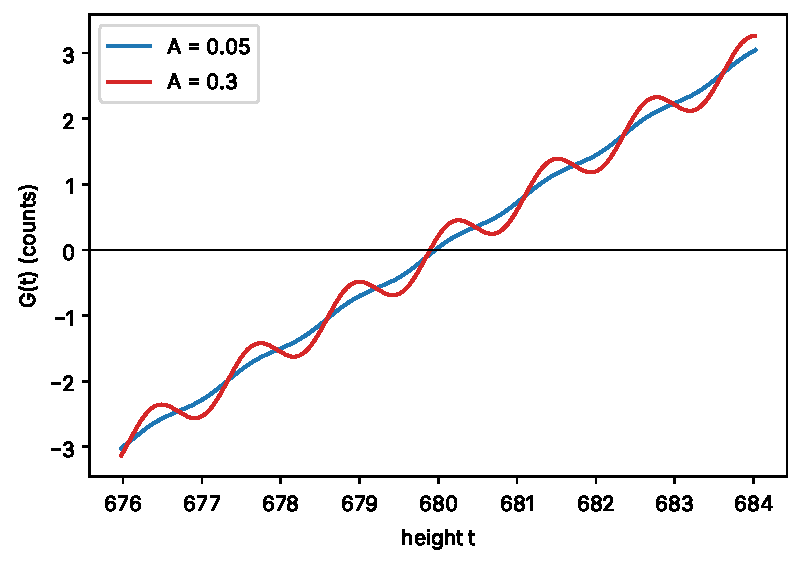
\includegraphics[width=0.85\linewidth]{figs/paper-arithmetic_rootambig.pdf}
\caption{Synthetic illustration of root ambiguity (not paper data). The level function $G(t)=\Nsm(t)-\Nsm(680)+A\sin(5t)$ is plotted over $680\pm3$ mean spacings for two amplitudes. For $A=0.05$, $|G'-\Nsm'|\le0.25<\Nsm'\approx0.75$ and the root is unique. For $A=0.3$, $A\omega=1.5$ exceeds $\Nsm'$, $G$ is not monotone, and the level equation has several roots in the bracket. A true counting function is a nondecreasing staircase, so several roots signal that $F$ is not behaving like a count.}
\label{fig:paper-arithmetic-rootambig}
\end{figure}

\begin{sample}{How big must a single wiggle be to create extra roots?}
Let $F(t)=A\sin(\omega t)$ with $\omega=5$, near $t=680$. Find the smallest $A$ for which $G(t)=\Nsm(t)+F(t)-c$ can fail to be monotone.

\textbf{Step 1: the slope.} $G'(t)=\Nsm'(t)+A\omega\cos(\omega t)$. Its smallest value over a cycle is $\Nsm'(t)-A\omega$.

\textbf{Step 2: the condition.} $G$ is monotone for all phases iff $A\omega<\Nsm'(t)$. At $t=680$, $\Nsm'=0.7455$ (Sample Problem "One oracle step by hand", Step 2).

\textbf{Step 3: solve.} $A>0.7455/5=0.149$.

\[
\boxed{A_{\min}\approx0.149}
\]
An amplitude of $0.15$ is smaller than the amplitude of the $p=2$, $m=1$ oracle term ($0.225$). High frequencies make wiggles cheap: the slope grows with $\omega$. An underdetermined fit with many frequencies up to $3\log863\approx20.3$ does not need large amplitudes to break monotonicity.
\end{sample}

\textbf{(d) Strength and limits.} The paper reports the row with its caveat attached, and the caveat is quantified: at most $0.012$. Even at the worst choice of root the score would be at most $0.192$, still far below the null $0.263$. The qualitative point of the row, that a badly underdetermined model built from the right frequencies still predicts with positive correlation, survives the ambiguity. The row is not a clean predictive score, and the paper says so.

\begin{checkpoint}
Control B with 900 coefficients on 400 zeros is underdetermined, and so is control C1. Why does B still reach $0.180$ while C1 stays at $0.258$?
\end{checkpoint}
\checkanswer{Both pick, among infinitely many exact fits, one regularized combination of their columns. In B every column is a correct arithmetic frequency, so any combination continues in roughly the right way beyond the window. In C1 the columns are a uniform grid that does not contain the arithmetic frequencies exactly; combinations that fit the window do not continue correctly. Same count, same underdetermination, different vocabulary.}

\begin{keyideas}
\item Given the frequencies, amplitudes are easy to learn: 150 coefficients from 400 zeros give $0.028$, better than the unfitted 25-prime oracle.
\item Underdetermination (900 unknowns, 400 equations) degrades B to $0.180/+0.78$, still well below the null.
\item Root ambiguity arises when $|F'|$ exceeds $\Nsm'$; for this row it changes the score by at most $0.012$.
\end{keyideas}

%======================================================================
\section{Control C1: a dense uniform grid of frequencies}\label{sec:paper-arithmetic-C1}

\textbf{(a) Plain words.} C1 has no arithmetic input: 450 frequencies on a uniform grid, $\omega_j=8j/450$ for $j=1,\dots,450$ (Appendix~A step 20), with sine and cosine amplitudes fitted by ridge: 900 coefficients. The paper: it "stays within $0.005$ of the null ($0.258$, correlation $+0.28$ with interval $[+0.08,+0.46]$): capacity without a suitable prior does not generalize, and in this respect the operator family is not special." On 801--1000 it scores $0.267/+0.22$ against a null of $0.274$. Its rms interval on 401--500 is $[0.231,0.285]$, which contains the null.

\textbf{(b) Tools.} Fourier resolution (Chapter~\ref{ch:fourier-transform}); ridge filter factors (Chapter~\ref{ch:least-squares}); the dense-grid control (Chapter~\ref{ch:sparse-frequency}).

\textbf{(c) Computation and analysis.} Recall from Chapter~\ref{ch:fourier-transform} that a window of length $T$ resolves frequencies separated by about $2\pi/T$. For the training window of zeros 1--400, $T=t_{400}-t_1\approx666$, so $2\pi/T\approx0.0094$. The grid spacing is $8/450=0.0178$, about $1.9$ resolution widths. A grid of this spacing does not contain the arithmetic frequencies; it contains nearby ones.

\begin{sample}{How far is each arithmetic frequency from the C1 grid?}
For $\log2$, $\log3$ and $\log5$, find the nearest grid frequency $\omega_j=8j/450$, the offset $\delta\omega$, and the phase drift $\delta\omega\,T$ accumulated across the training window.

\textbf{Step 1: $\log 2=0.693147$.} $0.693147\times450/8=38.99$, so $j=39$ and $\omega_{39}=0.693333$; $\delta\omega=0.000186$; drift $0.000186\times666=0.12$ rad.

\textbf{Step 2: $\log3=1.098612$.} $1.098612\times56.25=61.80$, so $j=62$, $\omega_{62}=1.102222$; $\delta\omega=0.00361$; drift $2.4$ rad.

\textbf{Step 3: $\log5=1.609438$.} $1.609438\times56.25=90.53$, so $j=91$, $\omega_{91}=1.617778$; $\delta\omega=0.00834$; drift $5.6$ rad, almost a full cycle.

\[
\boxed{\text{drifts across the window: } 0.12,\ 2.4,\ 5.6\ \text{rad for } \log2,\ \log3,\ \log5}
\]
A single grid column cannot follow the $p=5$ term across the window, because it slips nearly a whole cycle. The fit can still mimic the $p=5$ term inside the window by combining several neighboring columns, the way two nearby tones produce beats (first-year physics). But that combination is tuned to the window, and its continuation outside is a different beat pattern, not the $p=5$ term.
\end{sample}

This analysis is our reading of one mechanism, not the paper's stated explanation. The paper's own statement is more general: "capacity without a suitable prior does not generalize." Two further mechanisms point the same way. First, 900 coefficients on 400 zeros is underdetermined, so the fit chooses among infinitely many exact interpolants. Second, the forward split then selects a ridge strength. Recall the ridge filter: the coefficient along the $i$-th singular direction is multiplied by $\sigma_i/(\sigma_i^2+\lambda\sigma_1^2)$ instead of $1/\sigma_i$. For $\lambda\sigma_1^2\gg\sigma_i^2$ the factor is about $\sigma_i/(\lambda\sigma_1^2)$, tiny. If the validation block shows that the unregularized interpolant extrapolates badly, the selected $\lambda$ is large and the predictions shrink toward zero, that is, toward the null. Sample Problem "Reading a correlation off an rms" showed that C1's $0.258$ is close to the best rms ($0.252$) compatible with its correlation of $+0.28$: a weak, heavily shrunk prediction.

\textbf{(d) Strength and limits.} C1 is the cleanest answer to the parameter-count question: same count as the largest operator (900), same underdetermination, a basis that is even "Fourier" in name, and no skill to speak of. In Sec.~VI the paper summarizes: "a dense 900-coefficient Fourier model gains almost nothing over the null." Note the word "almost". C1's correlation interval, $[+0.08,+0.46]$, excludes zero, which no operator row in Table~I achieves reproducibly; C1 does extract a weak positive signal. The paper's statement that "in this respect the operator family is not special" refers to generalization of rms, where C1, like the operators, stays at the null.

\begin{checkpoint}
Suppose a reader says: "C1 failed because 450 frequencies are too few to cover $[0,8]$." Using control C2's result, how would you reply?
\end{checkpoint}
\checkanswer{C2 uses only $24$ frequencies on the same range and predicts at $0.034$. The issue is not how many frequencies, but whether they are the right ones, placed precisely. A dense grid spends its budget everywhere; a sparse search spends it where the data's spectrum actually has power.}

%======================================================================
\section{Control C2: a sparse frequency search with no arithmetic input}\label{sec:paper-arithmetic-C2}

\subsection{The algorithm, line by line}

Sec.~II~D describes C2 as "a sparse model whose $K$ frequencies are found one at a time as the largest peak of the periodogram of the current residual on $0.05<\omega<8$, with all amplitudes refitted after each addition ($3K$ parameters)." Appendix~A step 20 adds the details: "sparse search with step a quarter of $2\pi/T$, refinement on 201 points, joint refit after each added frequency, $K\le\min(300,n_{\rm fit}/3)$." Unpacked:

\begin{enumerate}
\item \emph{Start.} Residual $r_n=y_n$ at the training zeros, Eq.~\eqref{eq:paper-arithmetic-yn}; no frequencies selected.
\item \emph{Periodogram.} Recall from Chapter~\ref{ch:fourier-transform} the periodogram for irregular samples, $\mathcal P(\omega)=\bigl|\sum_n r_n e^{-i\omega t_n}\bigr|^2$. It is large at $\omega$ when $r_n$ contains a sinusoid of that frequency, because the phases $e^{-i\omega t_n}$ then cancel the oscillation of $r_n$ and the terms add coherently.
\item \emph{Coarse search.} Evaluate $\mathcal P$ on a grid over $0.05<\omega<8$ with step $\tfrac14\cdot2\pi/T=\pi/(2T)$. For $T\approx666$ the step is $0.00236$, so the grid has about $3370$ points. With four grid points per resolution width, every peak (width about $2\pi/T$) is sampled several times, so the coarse maximum is unlikely to miss a peak; the refinement step then locates it precisely. (This makes a miss unlikely; it does not strictly guarantee against one, for example when two peaks of nearly equal height compete.)
\item \emph{Refinement.} Around the coarse maximum, search $201$ finer points and take the maximum there. (The exact refinement interval is in the reconstruction record \cite{zenodo}.)
\item \emph{Joint refit.} Add the refined frequency to the list and refit \emph{all} amplitudes $a_j,b_j$ of all selected frequencies together by least squares. Update $r_n$ to the new residual. The joint refit matters: two nearby sinusoids leak into each other's periodogram peaks, and refitting them together removes the leakage that a one-at-a-time subtraction would leave.
\item \emph{Repeat} up to $K_{\max}=\min(300,n_{\rm fit}/3)$: $133$ for 400 training zeros, $266$ for 800. The cap $n_{\rm fit}/3$ ensures $3K\le n_{\rm fit}$, so the final fit is never underdetermined.
\item \emph{Select $K$ and ridge} by the forward split, then refit on the whole window.
\end{enumerate}

Step 5 is the connection to matching pursuit (Chapter~\ref{ch:sparse-frequency}): pick the best single atom, refit, repeat.

\begin{pycode}
import numpy as np, qmnt
t = qmnt.zeros(400); n = np.arange(1, 401)
y = n - 0.5 - qmnt.Nsm(t)                       # targets y_n
T = t[-1] - t[0]                                # training window length
d = 0.25*2*np.pi/T                              # coarse step
coarse = np.arange(0.05, 8.0, d)
def design(w):
    return np.hstack([np.sin(np.outer(t, w)), np.cos(np.outer(t, w))])
def peak(r, grid):                              # largest periodogram peak
    Pw = np.abs(np.exp(-1j*np.outer(grid, t)) @ r)**2
    return grid[np.argmax(Pw)]
freqs, r = [], y.copy()
for step in range(10):
    w0 = peak(r, coarse)
    w1 = peak(r, np.linspace(w0 - d, w0 + d, 201))   # refinement
    freqs.append(w1)
    X = design(np.array(freqs))
    coef, *_ = np.linalg.lstsq(X, y, rcond=None)      # joint refit
    r = y - X @ coef
print(np.round(freqs, 4))
print(np.round(np.exp(freqs), 2))               # compare with prime powers
\end{pycode}

The listing omits ridge and the choice of $K$, which only matter once many frequencies have been selected. Running it, the first frequency selected is within $\pi/T$ of $\log2$, and each of the first five lies within $\pi/T$ of the logarithm of a prime power (CHECKS). The last line prints $e^{\omega}$, which for a matched frequency is close to the prime power $q$ itself. \cref{fig:paper-arithmetic-periodogram} shows the periodogram that the very first step sees.

\begin{figure}[htbp]\centering
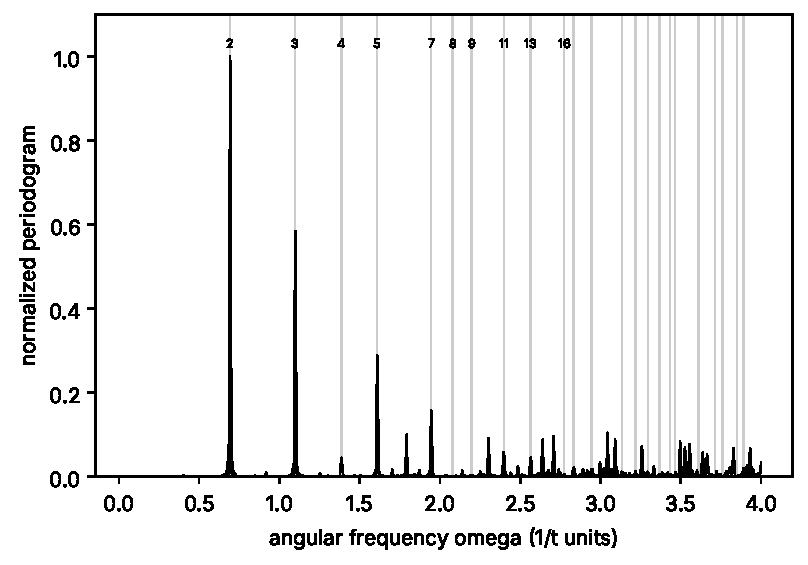
\includegraphics[width=0.85\linewidth]{figs/paper-arithmetic_periodogram.pdf}
\caption{Periodogram $\mathcal P(\omega)=|\sum_n y_n e^{-i\omega t_n}|^2$ of the targets $y_n=n-\tfrac12-\Nsm(t_n)$ at the first 400 zeros, normalized to its maximum, for $0.05<\omega<4$ (angular frequency in units of inverse height $t$). Vertical lines mark $\log q$ for prime powers $q\le 50$, labeled for $q\le 16$. The tallest peak sits at $\log 2$, and the next tallest are at logarithms of other small prime powers: the first step of control C2 sees the primes without being told about them.}
\label{fig:paper-arithmetic-periodogram}
\end{figure}

\subsection{What C2 found}

The paper (Sec.~IV): C2 "selects 24 frequencies (72 parameters) from 400 zeros and predicts zeros 401--500 at $0.034$ with correlation $+0.99$, the level of the 25-prime oracle; from 800 zeros it selects 43 frequencies and scores $0.034$/$+0.99$ on 801--1000." The bootstrap interval on 401--500 is $[0.028,0.041]$ (Table~IV caption). Then: "Every selected frequency lies within half the Fourier resolution of the training window of the logarithm of a prime power (for the 800-zero fit, 43 distinct prime powers: those up to 113 except 32, 64, and 81, and six primes between 131 and 211)."

"Half the Fourier resolution" is $\tfrac12\cdot2\pi/T=\pi/T$, the matching criterion $|\omega-\log q|<\pi/T$ of Appendix~A step 23. For the 800-zero window, $T=t_{800}-t_1\approx1170$, so $\pi/T\approx0.0027$.

\begin{sample}{Checking the list of 43 prime powers}
(a) Verify that "prime powers up to 113 except 32, 64, 81, plus six primes" makes 43. (b) Compute the weights $w(q)=1/(mp^{m/2})$ of the excluded and of some included prime powers, and see whether weight explains which were found.

\textbf{Step 1: primes up to 113.} There are $30$ of them ($2,3,\dots,109,113$).

\textbf{Step 2: higher prime powers up to 113.} $4,8,16,32,64$; $9,27,81$; $25$; $49$. ($121=11^2$ exceeds 113.) That is $10$.

\textbf{Step 3: count.} $30+10-3+6=43$. \checkmark

\textbf{Step 4: weights of the excluded ones.} $w(32)=1/(5\cdot2^{5/2})=0.0354$; $w(64)=1/(6\cdot8)=0.0208$; $w(81)=1/(4\cdot9)=0.0278$.

\textbf{Step 5: weights of the faintest included ones.} $w(16)=1/(4\cdot4)=0.0625$; $w(211)=1/\sqrt{211}=0.0688$; $w(113)=0.0941$.

\[
\boxed{30+10-3+6=43;\quad \text{excluded: } w\le0.0354;\quad \text{included: } w\ge0.0625}
\]
Up to $113$ the separation is clean: every prime power of weight at least $0.0625$ was found, and the three of weight at most $0.0354$ were not. Weight is not the whole story, however. All 17 primes from $127$ to $211$ have $w\ge0.0688>w(16)$, yet only six were found. At higher frequency the logarithms of neighboring primes crowd together: $\log139-\log137=0.0145$, only $2.7$ resolution widths $2\pi/T\approx0.0054$, and $\log128-\log127=0.0078$, only $1.5$. A finite window struggles to separate them. Note also that $16=2^4$ has $m=4$, beyond the $m\le3$ of Eq.~\eqref{eq:paper-arithmetic-nfl}: C2 found a term the oracle omits, as the untruncated explicit formula says it should. The paper does not say which six primes were selected, so we cannot test this reading further.
\end{sample}

\begin{checkpoint}
C2 at $0.034$ beats the 25-prime oracle ($0.043$) on zeros 401--500, although it was never told about primes. Give two reasons this is possible.
\end{checkpoint}
\checkanswer{First, it fits amplitudes, which (as control B showed) helps relative to the sharply truncated exact amplitudes. Second, it is not limited to the 75 frequencies $m\log p$ with $p\le97$, $m\le3$: it can pick, for example, $\log16$ ($m=4$) if the data demand it. Its 24 frequencies are chosen where the residual has the most power.}

\begin{keyideas}
\item C2: greedy periodogram peaks on $0.05<\omega<8$, quarter-resolution coarse grid, 201-point refinement, joint refit, $K\le\min(300,n_{\rm fit}/3)$; $K$ and ridge by forward split.
\item With $72$ parameters and no arithmetic input it predicts at $0.034/+0.99$, the level of the 25-prime oracle.
\item Its frequencies match $\log p^m$; which prime powers it finds is explained partly by their weights $1/(mp^{m/2})$ and partly by resolution.
\end{keyideas}

%======================================================================
\section{Is the alignment real? The surrogate check}\label{sec:paper-arithmetic-surrogate}

\subsection{Why a check is needed}

"Every selected frequency lies near $\log p^m$" sounds decisive. But the frequencies are the \emph{output of a search}, and the logarithms of prime powers are not sparse at large $\omega$. A frequency chosen at random could land near some $\log q$ by chance. How likely is that?

\begin{sample}{The chance that a random frequency matches some prime power (heuristic)}
Estimate the expected number $\lambda(\omega)$ of prime powers $q$ with $|\omega-\log q|<\pi/T$, for the 400-zero window ($2\pi/T\approx0.0094$), at $\omega=2$, $\omega=\log113$ and $\omega=8$, and the probability of at least one match.

\textbf{Step 1: density of $\log q$.} By the prime number theorem (Chapter~\ref{ch:primes}), the number of primes in $[x,x+\dd x]$ is about $\dd x/\log x$. With $x=e^\omega$, $\dd x=e^\omega\dd\omega$, so the number of $\log p$ in $[\omega,\omega+\dd\omega]$ is about $e^\omega\dd\omega/\omega$. Higher prime powers are much rarer, and we neglect them.

\textbf{Step 2: expected count.} The matching window has width $2\pi/T$, so $\lambda(\omega)\approx(2\pi/T)\,e^\omega/\omega$.

\textbf{Step 3: evaluate.} $\omega=2$: $0.0094\times7.389/2=0.035$. $\omega=\log113=4.727$: $0.0094\times113/4.727=0.23$. $\omega=8$: $0.0094\times2981/8=3.5$.

\textbf{Step 4: probability of at least one match.} Treating the $\log q$ as scattered at random (a heuristic), $\Pr\approx1-e^{-\lambda}$: $0.034$, $0.20$, $0.97$.

\[
\boxed{\Pr(\text{chance match})\approx0.034\ (\omega=2),\quad0.20\ (\omega=\log113),\quad0.97\ (\omega=8)}
\]
Near $\omega=8$ almost any frequency "matches a prime power" ($e^8\approx2981$, which is why the matching uses $q\le3000$). At low $\omega$ a chance match is rare. So a list of matches is impressive mainly for its low-frequency members, and how impressive it is overall depends on details that only a careful null can settle. This is a back-of-envelope estimate, not the paper's statistic.
\end{sample}

There is a second, subtler worry. The \emph{procedure} itself, periodogram peaks of a residual sampled at the zeros, might prefer certain frequencies for reasons unrelated to the signal. Recall from Chapter~\ref{ch:explicit-formula} Landau's formula: sums like $\sum_n e^{-i\omega t_n}$ over the zeros themselves peak at $\omega=\log p^m$ \cite{landau,gonek}. Since the zeros are the sample points, one must rule out that the alignment is produced by the sampling rather than by the target.

\subsection{What the paper did}

The paper: "Because the frequencies are the output of a search, this alignment was checked by rerunning the complete procedure on surrogate zero sets: phase-randomized surrogates and two families of sparse signals with non-arithmetic frequencies, 900 replicates in all. None approaches the alignment of the real zeros." Appendix~A step 23 gives the composition: 200 replicates of each family for the 400-zero fit and 100 of each for the 800-zero fit, so $3\times200+3\times100=900$. The three families are:

\begin{itemize}
\item \emph{Sorted phase-randomized surrogates} (Chapter~\ref{ch:controls}, \cite{theiler}): same power spectrum as the real fluctuation sequence, phases scrambled, no arithmetic content in the phases; "sorted" so that the surrogate zeros form an increasing sequence.
\item \emph{Explicit formulas with 25 displaced prime frequencies}: signals with the explicit formula's sparse structure but with each $\log p$ moved off its arithmetic value.
\item \emph{Explicit-formula shapes with 25 random base frequencies}: the same kind of sparse, harmonic structure built on random base frequencies.
\end{itemize}
The two sparse families are the sharp controls: they look like the real signal in every respect except arithmetic. If C2 still returned frequencies near $\log q$ on them, the alignment would be an artifact of the search or of the sampling.

The result is reported as a "cutoff-maximized binomial score $24.7$ and $50.9$ on the real zeros, at most $4.7$ on surrogates (score defined after the data were seen)." The construction of the score, which does not depend on a chosen frequency cutoff, is documented in the reconstruction record \cite{zenodo}; the paper's text does not give the formula, and we do not guess it.

\subsection{The status of the check}

The paper attaches two explicit qualifications, and you should keep both.
\begin{enumerate}
\item "The statistic was defined after the data were seen, so the check is exploratory." Recall from Chapter~\ref{ch:controls}: once a statistic has been chosen while looking at the result, its value on the real data cannot be turned into a significance level, because the choice itself may have favored the data.
\item "No significance claim is made here beyond the size of the ensembles." With $N$ surrogates of one family and none reaching the real value, the most a permutation-style argument could ever give is an empirical tail probability of about $1/(N+1)$; for $N=200$ that is about $0.005$. The paper does not even claim this, because of qualification 1.
\end{enumerate}

\begin{pitfall}
Do not describe C2 as "discovering the primes in the zeros". The paper is explicit: "That the Fourier transform of the zeros is concentrated at logarithms of prime powers is classical \cite{landau,gonek}; C2 is a control built on that fact, not a new result, and `sparse in $t$-frequency' is itself a strong and well-chosen prior." C2's role is to show that a fitting procedure \emph{can} learn the transferable structure from 400 zeros when its prior is right; it is not a claim about number theory.
\end{pitfall}

\begin{checkpoint}
Suppose, on the "displaced prime frequency" surrogates, C2 had returned frequencies near the true $\log p$ rather than near the displaced ones. What would that have meant?
\end{checkpoint}
\checkanswer{That the procedure is drawn to $\log p$ regardless of the target, for example through the sampling at the zeros (Landau's peaks) or through the matching tolerance. The alignment on the real zeros would then be an artifact, not evidence that C2 learned the target's frequencies. The paper reports that no surrogate approached the real alignment.}

%======================================================================
\section{Dephasing: why C2's skill fades with distance}\label{sec:paper-arithmetic-dephase}

\textbf{(a) Plain words.} The paper: "Its skill also decays with distance from the training window as the estimated frequencies dephase ($0.078$/$+0.96$ on zeros 1001--2000 for the 400-zero fit), which the exact frequencies of the oracle do not." Compare Table~V on the same holdout: six primes $0.091$, twenty-five primes $0.054$. On 401--500 C2 beat the 25-prime oracle ($0.034$ against $0.043$); on 1001--2000 it has fallen behind it ($0.078$ against $0.054$).

\textbf{(b) Tools.} Frequency estimation from a finite window (Chapters~\ref{ch:fourier-transform} and \ref{ch:sparse-frequency}).

\textbf{(c) The mechanism, derived.} Suppose the true term is $a\sin(\omega t)$ and the model has learned $a\sin(\hat\omega t+\hat\phi)$ with $\hat\omega=\omega+\delta\omega$. Least squares pins the phase where the data are, roughly at the window center $t_c$, so write the learned term as $a\sin\bigl(\omega t+\varphi(t)\bigr)$ with
\begin{equation}
\varphi(t)=\delta\omega\,(t-t_c).
\label{eq:paper-arithmetic-phase}
\end{equation}
The error from this one term is, by the identity $\sin X-\sin Y=2\cos\frac{X+Y}{2}\sin\frac{X-Y}{2}$,
\begin{equation}
e(t)=a\bigl[\sin(\omega t+\varphi)-\sin(\omega t)\bigr]
=2a\cos\!\Bigl(\omega t+\tfrac{\varphi}{2}\Bigr)\sin\tfrac{\varphi}{2}.
\label{eq:paper-arithmetic-deperr}
\end{equation}
Over one cycle, the mean square of $\cos$ is $\tfrac12$, and $\varphi$ hardly changes during a cycle, so the rms error is
\begin{equation}
e_{\rm rms}(t)=\sqrt2\,a\,\Bigl|\sin\frac{\varphi(t)}{2}\Bigr| \approx \frac{a}{\sqrt2}\,|\delta\omega|\,|t-t_c|\quad(\varphi\ll1).
\label{eq:paper-arithmetic-deprms}
\end{equation}
The error grows linearly with distance from the window center until $\varphi$ approaches $\pi$, where the learned term is fully out of phase. The oracle's frequencies are exact, $\delta\omega=0$, so it suffers no dephasing at all; its slow decline in Table~V has the different cause discussed in \cref{sec:paper-arithmetic-tablev}. \cref{fig:paper-arithmetic-dephase} shows the effect with an exaggerated frequency error.

\begin{figure}[htbp]\centering
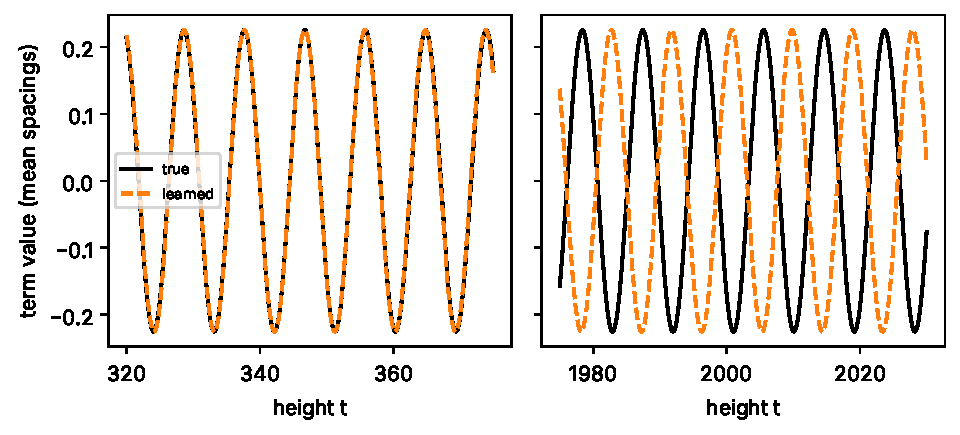
\includegraphics[width=0.95\linewidth]{figs/paper-arithmetic_dephase.pdf}
\caption{Dephasing of a learned frequency (synthetic; the frequency error is exaggerated for visibility). Black: the true $p=2$ term $a\sin(t\log2)$ with $a=1/(\pi\sqrt2)$, in mean spacings. Orange dashed: a learned copy with frequency error $\delta\omega=2\times10^{-3}$, phase pinned at the training-window center $t_c=347$. Left: near the window center the two agree. Right: at $t\approx2000$, about 1650 units of $t$ away, the phase error $\varphi=\delta\omega(t-t_c)$ is about $3.3$ rad and the learned term is nearly inverted.}
\label{fig:paper-arithmetic-dephase}
\end{figure}

\begin{sample}{How fast does one dephased term lose skill?}
Take the dominant term, $p=2$, $m=1$, with amplitude $a=1/(\pi\sqrt2)=0.225$ mean spacings (by Eq.~\eqref{eq:paper-arithmetic-predfluct}, amplitudes of $\Nfl$ are amplitudes of the predicted fluctuation). Assume a hypothetical frequency error $\delta\omega=10^{-4}$. Compute the rms error at distances $|t-t_c|=400$ and $1600$.

\textbf{Step 1: phases.} $\varphi=10^{-4}\times400=0.04$ rad and $10^{-4}\times1600=0.16$ rad.

\textbf{Step 2: prefactor.} $\sqrt2\,a=\sqrt2/(\pi\sqrt2)=1/\pi=0.3183$.

\textbf{Step 3: errors.} $0.3183\sin(0.02)=0.0064$ and $0.3183\sin(0.08)=0.025$.

\[
\boxed{e_{\rm rms}\approx0.0064\ \text{at}\ 400,\qquad e_{\rm rms}\approx0.025\ \text{at}\ 1600}
\]
A fourfold increase in distance gives a fourfold increase in error, as Eq.~\eqref{eq:paper-arithmetic-deprms} predicts for small $\varphi$. The distances are representative: the training window 1--400 spans $t\approx14$ to $680$, so $t_c\approx347$; zeros 401--500 lie a few hundred units above it, and zeros 1001--2000 run from just above $t_{1000}=1419.42$ (paper Sec.~II~A) to about $t=2515$. The value of $\delta\omega$ is invented for illustration; the paper does not report C2's frequency errors.
\end{sample}

\begin{checkpoint}
The matching criterion allows $|\delta\omega|$ up to $\pi/T\approx0.0047$ for the 400-zero window. If C2's dominant frequency were off by that much, what would happen at $|t-t_c|=1600$? What does the observed correlation $+0.96$ on 1001--2000 then tell you?
\end{checkpoint}
\checkanswer{$\varphi\approx0.0047\times1600\approx7.6$ rad, more than a full cycle: the dominant term would be completely dephased and the prediction would have lost much of its skill. Since C2 still correlates $+0.96$ there, its dominant frequencies must be estimated far more precisely than the matching tolerance. The tolerance is a criterion for naming a frequency, not the accuracy actually achieved.}

\textbf{(d) Strength and limits.} The paper reports one far holdout (1001--2000) for C2; Sec.~VI notes that "the fitted sinusoidal controls were scored only below zero 2000." How C2 behaves at $n=10^4$, where the oracle is still at $+0.98$, is not measured. Dephasing is also what you should expect from any model that \emph{estimates} frequencies from a finite window; it is a quantitative cost of not knowing the arithmetic, and it shows that knowing it exactly (the oracle) is worth something that 400 zeros cannot fully supply.

\begin{keyideas}
\item A frequency error $\delta\omega$ produces a phase error $\delta\omega(t-t_c)$ that grows with distance from the training window, Eq.~\eqref{eq:paper-arithmetic-phase}.
\item The resulting rms error grows linearly at first, Eq.~\eqref{eq:paper-arithmetic-deprms}; exact frequencies do not dephase.
\item C2 falls from $0.034$ to $0.078$ between 401--500 and 1001--2000, while the oracle does not dephase.
\end{keyideas}

%======================================================================
\section{The obstacle is the parametrization, not the parameter count}\label{sec:paper-arithmetic-param}

\subsection{Assembling the argument}

Claim IV.10 appears in the abstract ("the obstacle is the parametrization, not the parameter count"), in Sec.~IV, and in Sec.~VI. Here is the argument, piece by piece, with its evidence.

\begin{enumerate}
\item \emph{Many terms are not harmful if they have the right form.} Control A improves to $0.018$ at 900 terms.
\item \emph{Many fitted parameters are not harmful if the prior is right.} Control B with 150 fitted coefficients reaches $0.028$; even underdetermined at 900, it stays far below the null ($0.180$, positively correlated).
\item \emph{Many fitted parameters with a generic prior do not generalize, whatever the basis.} C1 with 900 coefficients: $0.258$, within $0.005$ of the null. The operators with 400--900 coefficients: $0.279$ to $0.369$ in Table~IV, never below the null.
\item \emph{Few fitted parameters with a strong but non-arithmetic prior suffice.} C2 with 72: $0.034$.
\item \emph{The arithmetic frequencies need not be supplied.} C2 finds them.
\end{enumerate}

Put together: at a fixed count of 900, scores range from $0.018$ (A) through $0.180$ (B) and $0.258$ (C1) to $0.302$ (the $M=900$ operator, on 801--1000). And the best fitted model has only 72 parameters. Count does not organize the results; prior does. \cref{fig:paper-arithmetic-budget} shows the 401--500 column of Table~IV.

\begin{table}[htbp]\centering\small
\caption{Paper Table~IV, quoted exactly: rms / correlation on the first held-out window after the training zeros. "Fitted" counts fitted real parameters. Nulls: $0.263$ (401--500) and $0.274$ (801--1000). $^\dagger$Root-ambiguous.}\label{tab:paper-arithmetic-tableiv}
\begin{tabular}{lccc}
\toprule
model & fitted & fit 1--400, 401--500 & fit 1--800, 801--1000 \\
\midrule
operator, cosine, $M=400$ & 400 & 0.369 / $-0.07$ & \\
operator, cosine, $M=600$ & 600 & 0.313 / $-0.16$ & 0.279 / $-0.03$ \\
operator, cosine, $M=900$ & 900 & & 0.302 / $+0.08$ \\
A: oracle, 25 primes & 0 & 0.043 / $+0.99$ & 0.053 / $+0.98$ \\
A: oracle, 300 primes (900 terms) & 0 & 0.018 / $+1.00$ & 0.020 / $+1.00$ \\
B: 25 primes, amplitudes fitted & 150 & 0.028 / $+0.99$ & 0.040 / $+0.99$ \\
B: 150 primes, amplitudes fitted$^\dagger$ & 900 & 0.180 / $+0.78$ & 0.100 / $+0.94$ \\
C1: uniform frequency grid & 900 & 0.258 / $+0.28$ & 0.267 / $+0.22$ \\
C2: sparse frequency search & 72, 129 & 0.034 / $+0.99$ & 0.034 / $+0.99$ \\
\bottomrule
\end{tabular}
\end{table}

\begin{figure}[htbp]\centering
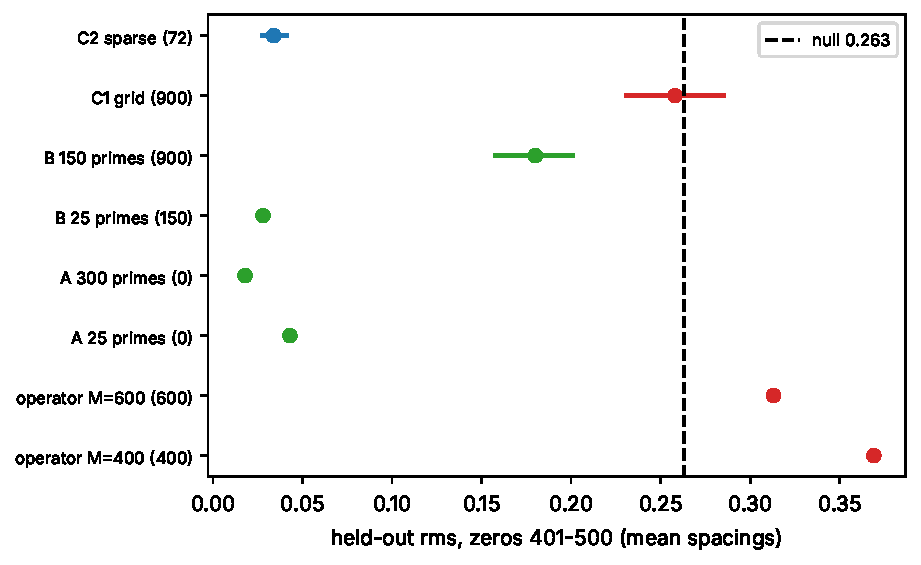
\includegraphics[width=0.85\linewidth]{figs/paper-arithmetic_budget.pdf}
\caption{Held-out rms on zeros 401--500 (fit on zeros 1--400) for every model of paper Table~IV with an entry in that column, colored by level of supplied information (green: arithmetic frequencies; blue: sparsity only; red: generic). Bars show the bootstrap 95\% intervals reported in the Table~IV caption where available. The dashed line is the null $0.263$. The number in each label is the count of fitted parameters; skill is unrelated to it.}
\label{fig:paper-arithmetic-budget}
\end{figure}

\subsection{"What fails is a potential $V(x)$ as the parametrization"}

The paper closes Sec.~IV: "The form is learnable from 400 zeros by a model told only that the fluctuation is a sum of few sinusoids in $t$; what fails is a potential $V(x)$ as the parametrization, as the continuation probe of Sec.~III shows from the other side." Recall the probe from Chapter~\ref{ch:paper-memorization}: trained on a pure $p=2$ oscillation (RE2) on levels 1--400, the operator family fits it in-sample (rms $0.056$, correlation $+0.95$) and continues it not at all on 401--500 (correlation $+0.07$). C2 and the probe are mirror images. C2: right vocabulary, the frequency is found from the data and continues. Probe: wrong vocabulary, the frequency is painted onto one window and does not continue.

Sec.~VI gives the heuristic reading, and labels it as heuristic: "the quantity being fitted is, by the explicit formula, an almost-periodic function of $t$ that is sparse in frequency, whereas a potential addresses the levels through their turning points, locally in energy." In the language of Chapters~\ref{ch:wkb} and \ref{ch:fourier-series}: a bump in $\delta V$ near the turning point $x_E$ shifts the levels whose energies turn near $x_E$, a local effect in level index; an almost-periodic function like $\sin(t\log2)+\sin(t\log3)$ never repeats (Chapter~\ref{ch:fourier-series}) and has no local description that implies its own continuation. A family that addresses levels locally can match a window but has no reason to extend it.

\subsection{Strengths and limits}

\textbf{Strengths.}
\begin{itemize}
\item The controls vary prior and count separately, on the same targets, splits and scoring as the operators, with the same null.
\item Held-out data are provably unused before scoring (the bit-identical test of Appendix~A step 20).
\item Bootstrap intervals are given for the decisive rows (A, B, C1, C2 on 401--500).
\item The one surprising positive result, C2's alignment with $\log p^m$, was checked against 900 surrogates, and its post hoc status is stated.
\end{itemize}

\textbf{Limits} (most stated by the paper itself, Sec.~VI).
\begin{itemize}
\item The fitted controls were scored only below zero 2000; the operator fits use at most the first 1000 zeros.
\item The alignment statistic was defined after the data were seen; the check is exploratory and carries no significance claim.
\item The 900-coefficient B row is root-ambiguous; its score is not clean (though bounded within $0.012$).
\item "The obstacle is the parametrization" is supported for the parametrizations tested (one background, three bases, one optimizer protocol); Sec.~VI is explicit that "this is evidence about the tested parametrizations and optimizer together, not a statement about what a potential can represent," and that whether the memorization result can be derived "is an open problem."
\item C2's prior, sparsity in $t$-frequency, is itself informed by the classical fact it recovers; the paper calls it "strong and well-chosen".
\item The bootstrap intervals resample held-out levels independently, although fluctuations are serially correlated (Sec.~VI: "except where stated").
\end{itemize}

\begin{checkpoint}
A reader argues: "C2 only works because sparsity in frequency is secretly arithmetic knowledge, so the comparison with the operators is unfair." Is this objection fatal to Claim IV.10?
\end{checkpoint}
\checkanswer{No. The paper concedes that the prior is strong and well chosen, and builds on a classical fact. Claim IV.10 does not say the operators lack a fair chance; it says that their failure is not explained by parameter count, because C1 shows count without the right prior fails and C2 shows the right prior with few parameters succeeds. The objection sharpens the conclusion: the right prior matters, and a potential in a generic basis does not supply it.}

\begin{keyideas}
\item At a fixed 900 parameters or terms, scores range from $0.018$ to $0.302$; the best fitted model has 72 parameters.
\item Prior, not count, organizes Table~IV.
\item C2 and the continuation probe of Sec.~III show the same point from opposite sides; the explanation in terms of locality in energy versus sparsity in frequency is heuristic and labeled so.
\end{keyideas}

%======================================================================
\section{Paper connection}\label{sec:paper-arithmetic-paper}

This chapter is itself a reading of the paper; here we collect the exact correspondences so you can find every item in R1.

\begin{itemize}
\item \textbf{Abstract.} The sentences "By contrast, a truncation of the Riemann--von Mangoldt explicit formula with zero fitted parameters predicts held-out zeros with correlation up to $+0.99$ through zero $10^4$" and "Controls with fitted sinusoidal models show that the obstacle is the parametrization, not the parameter count" are Claims IV.1, IV.3 and IV.10 (\cref{sec:paper-arithmetic-tablev,sec:paper-arithmetic-param}).
\item \textbf{Sec.~I.} "The information needed to predict unseen zeros is available, but it is arithmetic; within the operator families tested, the fits do not recover it, although a model with a non-arithmetic sparsity prior does (Sec.~IV)." Fig.~1 (operator $-0.07$, six-prime oracle $+0.96$) is rerun in \cref{fig:paper-arithmetic-oraclefit}.
\item \textbf{Sec.~I~A, paragraph "Explicit formul\ae{} for the $n$-th zero".} The oracle is an "information-existence baseline" with no claimed novelty \cite{francaleclair,leclair}; Connes' prime-only construction \cite{connes26} is "on the arithmetic side of our comparison". We kept this framing in \cref{sec:paper-arithmetic-levels}.
\item \textbf{Sec.~II~D and Eq.~(4).} The oracle Eq.~\eqref{eq:paper-arithmetic-nfl} and level equation Eq.~\eqref{eq:paper-arithmetic-level}; paragraph "Fitted sinusoidal controls" defines A, B, C1, C2, the target $y_n$, and the 75/25 forward split (\cref{sec:paper-arithmetic-levels}).
\item \textbf{Sec.~II~A and Eq.~(1).} $\Nsm$, smooth zeros, and "all errors below are quoted in units of the local mean spacing", the scoring of \cref{sec:paper-arithmetic-oracle}.
\item \textbf{Sec.~IV, first paragraph.} Claims IV.1--IV.4 and the three levels of information (\cref{sec:paper-arithmetic-tablev,sec:paper-arithmetic-levels}).
\item \textbf{Sec.~IV, paragraph "Comparable budgets and fitted controls".} Controls A (\cref{sec:paper-arithmetic-A}), B and root ambiguity (\cref{sec:paper-arithmetic-B}), C1 (\cref{sec:paper-arithmetic-C1}), C2 (\cref{sec:paper-arithmetic-C2}), the surrogate alignment check (\cref{sec:paper-arithmetic-surrogate}), dephasing (\cref{sec:paper-arithmetic-dephase}), and the closing "what fails is a potential $V(x)$ as the parametrization" (\cref{sec:paper-arithmetic-param}).
\item \textbf{Table~IV.} Quoted as Table~\ref{tab:paper-arithmetic-tableiv}, plotted in \cref{fig:paper-arithmetic-budget}; its caption's bootstrap intervals A $[0.015,0.020]$, B $[0.158,0.201]$, C1 $[0.231,0.285]$, C2 $[0.028,0.041]$, and its dagger.
\item \textbf{Table~V.} Quoted as Table~\ref{tab:paper-arithmetic-tablev}, rerun with \texttt{qmnt}, plotted in \cref{fig:paper-arithmetic-tablev}; caption's six-prime intervals $[+0.95,+0.97]$ (401--500) and $[+0.91,+0.92]$ (5001--10000).
\item \textbf{Sec.~II~C, "Within-height splits".} "the null grows from $0.263$ to $0.296$ over Table~V", the first column of Table~\ref{tab:paper-arithmetic-tablev}.
\item \textbf{Sec.~III, "Arithmetic-continuation probe".} The mirror image of C2 (\cref{sec:paper-arithmetic-param}).
\item \textbf{Sec.~VI.} "It is not the parameter count \dots\ It is not that the arithmetic frequencies must be supplied"; the heuristic reading in terms of almost-periodic, frequency-sparse targets versus turning-point locality; the limits (controls scored only below zero 2000; bootstrap independence).
\item \textbf{Appendix~A step 8.} Oracle root finding: Brent bracketed $\pm3$ gaps around the smooth zero, bracket expanded on sign failure.
\item \textbf{Appendix~A step 20.} Ridge filter and $\lambda$ grid; C1 grid $\omega_j=8j/450$; C2 step, refinement, joint refit, $K\le\min(300,n_{\rm fit}/3)$; the bit-identical leakage test.
\item \textbf{Appendix~A step 23.} Surrogate families and replicate counts (200 and 100 each), matching criterion $|\omega-\log q|<\pi/T$, $q\le3000$, scores $24.7$ and $50.9$ against at most $4.7$, "score defined after the data were seen"; key anchors $K=24$ and $K=43$.
\item \textbf{References used in Sec.~IV.} \cite{landau,gonek} for the classical concentration of the zeros' Fourier transform at $\log p^m$; \cite{theiler,schreiber} for surrogates; \cite{zenodo} for the reconstruction record.
\end{itemize}

%======================================================================
\section{Summary}\label{sec:paper-arithmetic-summary}

\begin{itemize}
\item The oracle solves $\Nsm(t)+\Nfl(t)=n-\tfrac12$, Eqs.~\eqref{eq:paper-arithmetic-nfl}--\eqref{eq:paper-arithmetic-level}, with no fitted parameters and no zero data; its predicted fluctuation in mean spacings is $-\Nfl$ at the predicted zero, Eq.~\eqref{eq:paper-arithmetic-predfluct}.
\item The slope of $\Nfl$ is comparable with $\Nsm'=\frac{1}{2\pi}\log\frac{t}{2\pi}$, Eq.~\eqref{eq:paper-arithmetic-nsmprime}, so the level equation must be solved; uniqueness is guaranteed when $B_P<\Nsm'$, Eq.~\eqref{eq:paper-arithmetic-bound}.
\item Table~V: more primes always help; skill persists through zero $10^4$, with correlation nearly constant and the rms ratio drifting mildly (Table~\ref{tab:paper-arithmetic-ratio}). One prime beats the best operator by about $1.34$.
\item rms $\ge\sigma_Y\sqrt{1-\rho^2}$, Eq.~\eqref{eq:paper-arithmetic-rmsbound}, links the two scores.
\item The fitted controls fit $F$ of Eq.~\eqref{eq:paper-arithmetic-F} to $y_n$ of Eq.~\eqref{eq:paper-arithmetic-yn} by ridge least squares, with strength and $K$ chosen by a forward split.
\item A (0 fitted, 900 terms): $0.018$. B (150 fitted): $0.028$; B (900, underdetermined, root-ambiguous): $0.180$. C1 (900, generic grid): $0.258$, near the null. C2 (72, sparse search): $0.034$, frequencies at $\log p^m$, checked against 900 surrogates in an exploratory analysis.
\item Estimated frequencies dephase, Eqs.~\eqref{eq:paper-arithmetic-phase}--\eqref{eq:paper-arithmetic-deprms}; C2 falls to $0.078$ on 1001--2000 while the oracle does not dephase.
\item The obstacle is the parametrization, not the parameter count, for the families and optimizer tested; the explanation is heuristic.
\end{itemize}

%======================================================================
\section{Problems}\label{sec:paper-arithmetic-problems}

\begin{problemlist}
\prob{1}{Control B with the first 10 primes and $m=1,2,3$: how many frequencies and how many fitted real parameters does it have? Is it over- or underdetermined with 400 training zeros?}

\prob{1}{For the 800-zero training window, $T=t_{800}-t_1\approx1170$. Compute the Fourier resolution $2\pi/T$ and the matching tolerance $\pi/T$. Compare with the 400-zero values $0.0094$ and $0.0047$.}

\prob{1}{Using the $\{2\}$ column of Table~\ref{tab:paper-arithmetic-tablev}, compute for each holdout the fraction of the null error removed, $1-\mathrm{rms}/\mathrm{null}$.}

\prob{1}{Assign each of the following to level (i), (ii) or (iii) of \cref{sec:paper-arithmetic-levels}: the six-prime oracle; control B with 25 primes; C1; C2; the scale-1 cosine operator with $M=600$; the Chebyshev operator of Table~II.}

\prob{2}{Starting from the level equation \eqref{eq:paper-arithmetic-level}, derive the Newton iteration for the predicted zero, starting from $s_n$. Show that the first iterate is $s_n-\Nfl(s_n)/[\Nsm'(s_n)+\Nfl'(s_n)]$, and state when it reduces to $s_n-\gap_n\Nfl(s_n)$.}

\prob{2}{Compute the bound $B_P$ of Eq.~\eqref{eq:paper-arithmetic-bound} for $P=\{2,3\}$ and the height above which the two-prime oracle's root is guaranteed unique.}

\prob{2}{Control B with 900 coefficients has correlation $+0.78$ on zeros 401--500. Using Eq.~\eqref{eq:paper-arithmetic-rmsbound} with $\sigma_Y\approx0.263$, find the best rms consistent with that correlation and compare with the reported $0.180$.}

\prob{2}{Compute the weights $w(q)=1/(mp^{m/2})$ for $q=121,125,127,128,169$. Which of these would an amplitude-only argument predict C2 to find from 800 zeros? The paper reports that the six primes found above 113 lie between 131 and 211, so $127$ was not among them. Suggest a reason, using $\log128-\log127$ and the resolution $2\pi/T\approx0.0054$.}

\prob{2}{Use the heuristic of the Sample Problem in \cref{sec:paper-arithmetic-surrogate} to estimate the expected number of prime-power logarithms within $\pi/T$ of $\omega=\log211$, for the 800-zero window ($2\pi/T\approx0.0054$).}

\prob{2}{Repeat the dephasing Sample Problem with $\delta\omega=5\times10^{-5}$ at distance $|t-t_c|=1000$.}

\prob{2}{Using \texttt{qmnt}, reproduce the 401--500 row of Table~V (null and all four prime budgets). Then compute the six-prime oracle on zeros 1--400. Does a zero-parameter predictor have an "in-sample" score? What does your number mean?}

\prob{2}{Using \texttt{qmnt}, reproduce the 1001--2000 row of Table~V for $\{2\}$ and six primes, and compute their rms/null ratios. Compare with Table~\ref{tab:paper-arithmetic-ratio}.}

\prob{3}{Using numpy and \texttt{qmnt}, implement control B with 25 primes as in the listing of \cref{sec:paper-arithmetic-B}. Report your held-out rms and correlation on zeros 401--500, and compare your fitted sine and cosine amplitudes for $\log2$ with the oracle's $-1/(\pi\sqrt2)$ and $0$.}

\prob{3}{Using numpy and \texttt{qmnt}, run the C2 listing for 15 steps on zeros 1--400. For each selected $\omega$, find the nearest $\log q$ over prime powers $q\le3000$ and record whether $|\omega-\log q|<\pi/T$. Then extend your code to choose $K$ by the 300/100 forward split.}

\prob{2}{Using numpy and \texttt{qmnt}, compute the periodogram of $y_n$ for the first 400 zeros on $0.05<\omega<8$. Where is its tallest peak? Rerun with $y_n$ replaced by a random permutation of itself (seed 1) and describe the change.}

\prob{2}{For the C1 grid $\omega_j=8j/450$, find the nearest grid frequency to $\log7$, the offset, and the phase drift across a window of length $T\approx666$.}

\prob{2}{Appendix~A step 20 states: "Overwriting held-out data with noise before fitting leaves all fitted coefficients bit-identical." Explain exactly what this test rules out, and give one kind of information flow from the test set that it does \emph{not} rule out.}

\prob{2}{Appendix~A step 23 uses 200 replicates per surrogate family for the 400-zero fit. What is the smallest empirical tail probability that $200$ replicates could support, if none reached the real score? Why does the paper decline to quote such a number?}

\prob{1}{The 900-coefficient B row scores $0.180$ and "the score varies by at most $0.012$ with the choice of root." Give the range of possible scores and compare with the null.}

\prob{2}{\label{prob:paper-arithmetic-selberg}Using Selberg's variance $\frac{1}{2\pi^2}\log\log t$ from the \texttt{beyond} box in \cref{sec:paper-arithmetic-tablev}, predict the ratio of the null rms at $t=8000$ to that at $t=700$. Compare with the ratio $0.296/0.263$ of Table~V's first and last nulls, and say what the asymptotic formula neglects.}

\prob{3}{For $F(t)=A\sin(\omega t)$ near $t=680$ with $\omega=5$, find the smallest $A$ for which the level function can be non-monotone. For $A=0.3$, how many times can $G$ change direction within one period $2\pi/\omega$? Relate your answer to \cref{fig:paper-arithmetic-rootambig}.}

\prob{2}{C2 beats the 25-prime oracle on zeros 401--500 ($0.034$ vs.\ $0.043$) but loses to it on 1001--2000 ($0.078$ vs.\ $0.054$). Explain both facts with the material of \cref{sec:paper-arithmetic-C2,sec:paper-arithmetic-dephase}.}

\prob{3}{Show from the ridge filter factor $\sigma_i/(\sigma_i^2+\lambda\sigma_1^2)$ that, as $\lambda\to\infty$, every ridge prediction tends to $F\equiv0$, i.e.\ to the null. Show also that for $\lambda\to0$ and an underdetermined system the solution tends to the minimum-norm exact fit. Use these limits to explain why C1's validation-selected ridge leaves it near the null.}

\prob{2}{Compute the ratio of C2's rms on 1001--2000 to its rms on 401--500, and the same ratio for the 25-prime oracle, from the numbers quoted in \cref{sec:paper-arithmetic-dephase}. Which ratio reflects dephasing?}

\prob{1}{C1's held-out rms interval is $[0.231,0.285]$ and its correlation interval is $[+0.08,+0.46]$. In plain words, what does each interval say about C1 relative to the null?}

\prob{3}{(Research flavor.) Suppose C2's search range were restricted to $0.05<\omega<2$. Which prime powers could it find? Predict, without running, roughly where its held-out rms on 401--500 would fall relative to Table~V, and explain. Then, if you like, test your prediction with your code from Problem 14.}

\prob{2}{Suppose a revised paper reported that C1, unchanged, scored $0.05$ on zeros 401--500. Which sentence of Sec.~IV or Sec.~VI would this contradict, and would Claim IV.10 survive?}

\prob{2}{\label{prob:paper-arithmetic-rmsslope}Starting from Eq.~\eqref{eq:paper-arithmetic-dnfl}, show that the mean square of $\Nfl'(t)$ over a long range of $t$ is $\frac{1}{\pi^2}\sum_{p\in P}(\log p)^2\sum_{m=1}^3\frac{1}{2p^m}$. (Hint: the frequencies $m\log p$ are all distinct, so the cross terms average to zero, and each $\cos^2$ averages to $\tfrac12$.) Evaluate the rms for $P=\{2\}$ and for the six primes $p\le13$, and compare both with $\Nsm'(680)$.}
\end{problemlist}

%======================================================================
\section{Answers to selected problems}\label{sec:paper-arithmetic-answers}

\textbf{Problem 1.} $10\times3=30$ frequencies, each with a sine and a cosine amplitude: $60$ fitted parameters. With 400 equations it is overdetermined (more equations than unknowns), so least squares has a unique best fit if the columns are independent.

\textbf{Problem 2.} $2\pi/1170\approx0.0054$ and $\pi/1170\approx0.0027$. Both are about $0.57$ times the 400-zero values, because the window is about $1170/666\approx1.76$ times longer; resolution improves in proportion to window length.

\textbf{Problem 3.} $1-0.198/0.263=0.247$; $1-0.208/0.270=0.230$; $1-0.219/0.279=0.215$; $1-0.232/0.288=0.194$; $1-0.242/0.296=0.182$. A single prime removes about a quarter to a fifth of the null error at every height in the table.

\textbf{Problem 4.} Six-prime oracle: (i). B with 25 primes: (i). C1: (iii). C2: (ii). Cosine operator $M=600$: (iii). Chebyshev operator: (iii) (it is another generic basis for $\delta V$).

\textbf{Problem 5.} Let $G(t)=\Nsm(t)+\Nfl(t)-(n-\tfrac12)$. Newton's method is $t_{k+1}=t_k-G(t_k)/G'(t_k)$. At $t_0=s_n$, $G(s_n)=\Nfl(s_n)$ because $\Nsm(s_n)=n-\tfrac12$, and $G'(s_n)=\Nsm'(s_n)+\Nfl'(s_n)$. Hence $t_1=s_n-\Nfl(s_n)/[\Nsm'(s_n)+\Nfl'(s_n)]$. It reduces to $s_n-\gap_n\Nfl(s_n)$ when $|\Nfl'(s_n)|\ll\Nsm'(s_n)=1/\gap_n$. Sample Problem "One oracle step by hand" shows that this condition fails badly for one prime at $t=680$ ($0.34$ vs.\ $0.75$).

\textbf{Problem 7.} $0.263\sqrt{1-0.78^2}=0.263\times0.626=0.165$. The reported $0.180$ is above this bound, as it must be (to the extent that the null approximates $\sigma_Y$). The excess is consistent with an amplitude that is not optimally scaled, a nonzero mean error, or both; the paper does not say which, and the bound alone cannot tell them apart.

\textbf{Problem 9.} $\lambda\approx0.0054\times211/\log211=0.0054\times39.4\approx0.21$. So even the highest frequency in the 800-zero list had only about a one-in-five chance of a match by accident under this heuristic; many such matches together are hard to obtain by chance, which is the intuition the surrogate check tests properly.

\textbf{Problem 11.} You should get null $0.263$, and $0.198/+0.66$, $0.116/+0.90$, $0.074/+0.96$, $0.043/+0.99$ for 1, 3, 6, 25 primes, matching Table~V. The oracle is not fitted, so a score on zeros 1--400 is not "in-sample" in the sense of training; it is simply another holdout. It tells you how well the truncated formula works at lower heights, where it also performs well.

\textbf{Problem 13.} Your rms should be well below the six-prime oracle's $0.074$, of the same order as Table~IV's $0.028$, and your correlation above $0.95$; exact values depend on validation details. The fitted sine amplitude for $\log2$ should lie within about $0.05$ of $-0.225$, and the cosine amplitude within about $0.05$ of zero: the data recover the explicit formula's amplitude and phase for the dominant term.

\textbf{Problem 15.} The tallest peak lies within $\pi/T$ of $\log2=0.693$, with the next tallest at logarithms of other small prime powers (see \cref{fig:paper-arithmetic-periodogram}). For the permuted sequence the peaks at $\log q$ disappear: permutation keeps the values but destroys the ordering in $t$, and with it every coherent oscillation; the periodogram becomes an irregular, roughly flat noise floor.

\textbf{Problem 17.} It rules out any dependence of the fitted coefficients on the values of held-out zeros: if those values could influence the fit, replacing them by noise would change at least one coefficient. It does not rule out influence through \emph{design choices} made by the researchers after seeing held-out results (for example, choosing the frequency range $0.05<\omega<8$ or the step size because they worked well on the test set). That kind of leakage lives in the protocol's history, not in the code, and is addressed by fixing the protocol in advance and reporting it.

\textbf{Problem 19.} The score lies in $[0.168,0.192]$, entirely below the null $0.263$. The qualitative conclusion (positive skill despite underdetermination) does not depend on the root choice.

\textbf{Problem 21.} $G'(t)=\Nsm'(t)+A\omega\cos(\omega t)$ can become negative only if $A\omega>\Nsm'(680)=0.7455$, so $A>0.149$. For $A=0.3$, $A\omega=1.5>0.7455$, so $G'(t)=0.7455+1.5\cos(5t)$ is negative exactly when $\cos(5t)<-0.7455/1.5=-0.497$, which happens on one interval of each period, and positive on the rest. Hence $G'$ changes sign exactly twice per period: $G$ has one local maximum $G_{\max}$ (where $G'$ goes from positive to negative) and one local minimum $G_{\min}<G_{\max}$ (where it goes back). So $G$ changes direction twice per period. Extra roots: around one such excursion, $G=0$ has three roots (one on the rising stretch before the maximum, one on the falling stretch, one on the rising stretch after the minimum) if and only if $G_{\min}<0<G_{\max}$; otherwise it has at most one. Each excursion whose range straddles zero therefore adds exactly two extra roots, which is what the $A=0.3$ curve of \cref{fig:paper-arithmetic-rootambig} shows.

\textbf{Problem 23.} The ridge solution is $\theta=\sum_i \frac{\sigma_i}{\sigma_i^2+\lambda\sigma_1^2}(u_i^\top y)\,v_i$. As $\lambda\to\infty$ every factor tends to $0$, so $\theta\to0$ and $F\equiv0$: the prediction is the smooth zero, the null. As $\lambda\to0$ each factor tends to $1/\sigma_i$ for $\sigma_i>0$, and the sum runs only over nonzero singular values, which is the pseudo-inverse solution: the exact fit of minimum norm (Chapter~\ref{ch:least-squares}). For C1 the minimum-norm exact fit extrapolates poorly; the forward split detects this in the validation block and selects a large $\lambda$, which pushes the held-out predictions toward the $\lambda\to\infty$ limit, the null.

\textbf{Problem 25.} The rms interval contains the null $0.263$: C1's rms cannot be distinguished from predicting no fluctuation. The correlation interval excludes zero: its predictions are weakly but genuinely aligned with the truth. Together: a little information, almost no error reduction, as Eq.~\eqref{eq:paper-arithmetic-rmsbound} predicts for $\rho\approx0.28$.

\textbf{Problem 26.} The prime powers with $\log q<2$, i.e.\ $q<e^2\approx7.39$, are $2,3,4,5,7$. A C2 restricted to this range can capture the terms $\log2$, $\log4=2\log2$, $\log3$, $\log5$, $\log7$, i.e.\ a subset of the four-prime oracle, with fitted amplitudes. We would expect a held-out rms roughly between the 3-prime ($0.116$) and 6-prime ($0.074$) oracle entries of Table~V, since it captures more than three primes' main terms but misses $p=11,13$ and all higher terms. This is a heuristic expectation, not a result; the fitted amplitudes could do a little better.

\textbf{Problem 27.} It would contradict "A dense 900-coefficient Fourier model also stays near the null" (abstract) and "a dense 900-coefficient Fourier model gains almost nothing over the null" (Sec.~VI). Claim IV.10 would weaken: count without an arithmetic or sparsity prior would then have generalized, and the operators' failure could no longer be blamed on a generic parametrization in general, only on the potential specifically.
